% =====================================================================
% Guia do Projeto — Trabalho de Computação Gráfica 2026.2 (2ª etapa)
% Compilar dentro de guia/:  pdflatex GUIA_DO_PROJETO.tex  (2 vezes, por causa do sumário)
% ou:                        tectonic GUIA_DO_PROJETO.tex
% =====================================================================
\documentclass[11pt,a4paper]{article}

\usepackage[T1]{fontenc}
\usepackage[utf8]{inputenc}
\usepackage[brazilian]{babel}
\usepackage{lmodern}
\usepackage{microtype}
\usepackage[a4paper,top=2.3cm,bottom=2.3cm,left=2.3cm,right=2.3cm]{geometry}
\usepackage{amsmath,amssymb}
\usepackage{graphicx}
\usepackage{float}
\usepackage{booktabs}
\usepackage{tabularx}
\usepackage{longtable}
\usepackage{array}
\usepackage{enumitem}
\usepackage[table]{xcolor}
\usepackage{tikz}
\usetikzlibrary{arrows.meta,positioning,calc,shapes.geometric,angles,quotes,babel}
\usepackage[most]{tcolorbox}
\usepackage{listings}
\usepackage{caption}
\usepackage{subcaption}
\usepackage{fancyhdr}
\usepackage{titlesec}
\usepackage[colorlinks=true,linkcolor=azul,urlcolor=azul]{hyperref}

\graphicspath{{../relatorio/figuras/}}

% --- Cores ---
\definecolor{azul}{HTML}{12355B}
\definecolor{azulclaro}{HTML}{1F5C99}
\definecolor{fundo}{HTML}{F4F6FA}
\definecolor{laranja}{HTML}{E0A030}
\definecolor{verde}{HTML}{2A9D8F}
\definecolor{peao}{HTML}{E63946}
\definecolor{lapis}{HTML}{F4A261}
\definecolor{altere}{HTML}{2A9D8F}
\definecolor{martelo}{HTML}{A8DADC}
\definecolor{lixeira}{HTML}{C77DFF}

% --- Títulos ---
\titleformat{\section}{\Large\bfseries\color{azul}}{\thesection.}{0.5em}{}[{\color{azul!40}\titlerule}]
\titleformat{\subsection}{\large\bfseries\color{azulclaro}}{\thesubsection}{0.5em}{}
\titleformat{\subsubsection}{\normalsize\bfseries\color{azulclaro}}{\thesubsubsection}{0.5em}{}
\newcommand{\novasecao}{\clearpage}

% --- Cabeçalho e rodapé ---
\pagestyle{fancy}
\fancyhf{}
\fancyhead[L]{\small\color{gray}Guia do Projeto — Computação Gráfica 2026.2}
\fancyhead[R]{\small\color{gray}\leftmark}
\fancyfoot[C]{\small\thepage}
\renewcommand{\headrulewidth}{0.3pt}
\renewcommand{\sectionmark}[1]{\markboth{#1}{}}

\setlength{\parindent}{0pt}
\setlength{\parskip}{6pt}
\renewcommand{\arraystretch}{1.25}
\setlist{itemsep=2pt,topsep=4pt}

% --- Comandos ---
\newcommand{\code}[1]{\texttt{\detokenize{#1}}}
\newcommand{\arq}[1]{\textcolor{azulclaro}{\texttt{\detokenize{#1}}}}
\newcommand{\vetor}[1]{\mathbf{#1}}
\newcommand{\norm}[1]{\left\lVert #1 \right\rVert}

% --- Caixas ---
\newtcolorbox{enunciado}{enhanced,breakable,colback=laranja!8,colframe=laranja,
  boxrule=0pt,leftrule=3pt,arc=0pt,left=8pt,right=8pt,top=4pt,bottom=4pt,
  fontupper=\small}
\newtcolorbox{conceito}[1]{enhanced,breakable,colback=azul!4,colframe=azul!60,
  boxrule=0.6pt,arc=2pt,title={#1},fonttitle=\bfseries\small,
  coltitle=white,colbacktitle=azul!80,left=6pt,right=6pt}
\newtcolorbox{pergunta}[1]{enhanced,colback=white,colframe=azulclaro!50,
  boxrule=0.5pt,leftrule=3pt,arc=0pt,left=8pt,right=8pt,top=3pt,bottom=3pt,
  before upper={\textbf{\color{azul}P:~#1}\par\smallskip\textbf{R:}~}}

% --- Código ---
\lstset{
  language=Python, basicstyle=\ttfamily\footnotesize, backgroundcolor=\color{fundo},
  frame=leftline, framerule=2pt, rulecolor=\color{azulclaro}, xleftmargin=8pt,
  keywordstyle=\color{azul}\bfseries, commentstyle=\color{gray}\itshape,
  stringstyle=\color{verde!70!black}, showstringspaces=false, columns=fullflexible,
  breaklines=true, aboveskip=6pt, belowskip=6pt,
  literate={á}{{\'a}}1 {é}{{\'e}}1 {í}{{\'i}}1 {ó}{{\'o}}1 {ú}{{\'u}}1
           {ã}{{\~a}}1 {õ}{{\~o}}1 {ç}{{\c c}}1 {â}{{\^a}}1 {ê}{{\^e}}1
           {ô}{{\^o}}1 {à}{{\`a}}1 {É}{{\'E}}1 {→}{{$\rightarrow$}}1
}

\begin{document}

% =====================================================================
% CAPA
% =====================================================================
\begin{titlepage}
\centering
\vspace*{2cm}
{\color{azul}\rule{\linewidth}{2pt}}\\[0.6cm]
{\Huge\bfseries\color{azul} Guia do Projeto}\\[0.4cm]
{\Large Trabalho de Computação Gráfica 2026.2 — 2ª etapa}\\[0.3cm]
{\color{azul}\rule{\linewidth}{2pt}}\\[1.2cm]

{\large Funcionalidades, fluxo do pipeline, conceitos,\\ implementação e perguntas para a apresentação}\\[2cm]

\begin{tikzpicture}[scale=0.9]
  \foreach \c/\x in {peao/0,lapis/1.3,altere/2.6,martelo/3.9,lixeira/5.2}{
    \fill[\c] (\x,0) rectangle ++(1,1);
  }
\end{tikzpicture}\\[2cm]

\begin{minipage}{0.8\linewidth}\centering\small
Instituto Federal do Ceará — Campus Fortaleza\\
Engenharia da Computação — Computação Gráfica\\
Prof. Ajalmar Rocha Neto, Dr.
\end{minipage}

\vfill
{\small Todos os números deste guia (vértices, caixas, base da câmera, matrizes) foram obtidos\\
rodando o próprio código do projeto com a configuração atual.}
\end{titlepage}

\tableofcontents
\clearpage

% =====================================================================
\section{Visão geral e fluxo do pipeline}
% =====================================================================

O projeto é um \textbf{pipeline gráfico implementado do zero em Python}, sem OpenGL: toda a
matemática de transformações, câmera, projeção, iluminação e rasterização está escrita à mão com
NumPy. As únicas bibliotecas externas são:

\begin{table}[H]\centering\small
\begin{tabularx}{\linewidth}{@{}l X X@{}}
\toprule
\textbf{Biblioteca} & \textbf{Para quê} & \textbf{Permitido pelo enunciado?} \\
\midrule
\code{numpy} & vetores, matrizes, produto escalar e vetorial & sim (só álgebra) \\
\code{scikit-image} & \textbf{somente} a função \code{marching_cubes}, que gera a malha &
  sim: o item 1b diz ``não precisa implementar esse algoritmo, basta usar de alguma API'' \\
\code{matplotlib} & mostrar a imagem final (\code{imshow}) e os gráficos 3D de apoio & sim (só exibição) \\
\bottomrule
\end{tabularx}
\end{table}

\subsection{Arquivos e responsabilidades}

\begin{table}[H]\centering\small
\begin{tabularx}{\linewidth}{@{}l X c@{}}
\toprule
\textbf{Arquivo} & \textbf{Papel} & \textbf{Itens} \\
\midrule
\arq{primitives.py} & Formas implícitas (cilindro, cone, esfera, caixa, toro) e operações booleanas & 1 \\
\arq{modeling.py} & Os 5 objetos, Marching Cubes, normais, arestas $\Rightarrow$ ``sólido completo'' & 1 \\
\arq{math_3d.py} & Matrizes $4\times4$ ($T$, $R$, $S$), base da câmera, look-at, projeção, recorte, culling & 2, 3, 4, 6 \\
\arq{cena.py} & Posição, rotação e escala de cada objeto; câmeras; luz; validação da cena & 2, 3, 5 \\
\arq{illumination.py} & Modelo de Phong (ambiente + difusa + especular) & 5 \\
\arq{rasterizer.py} & Equação da reta, scan-line par-ímpar, coordenadas baricêntricas & 6 \\
\arq{main.py} & Junta tudo: renderiza a cena em 200, 400 e 800 px e com um 2º eye & 3e, 4, 5, 6 \\
\arq{visualizar_objetos.py} & Cada sólido no seu sistema do objeto, com normais & 1e \\
\arq{visualizar_cena.py} & Todos os sólidos no sistema do mundo & 2b \\
\arq{visualizar_camera.py} & A cena no sistema da câmera, eixos $u, v, n$, origem do mundo & 3a--3e \\
\arq{visualizar_projecao.py} & Sólidos 3D + seus polígonos projetados na janela & 4a \\
\bottomrule
\end{tabularx}
\end{table}

\subsection{O caminho de um vértice, do começo ao fim}

A Figura~\ref{fig:pipeline} mostra os sistemas de coordenadas por onde cada vértice passa e a
transformação que leva de um para o outro. A função que executa os estágios por face é
\code{renderizar_cena_completa} (\arq{main.py:110}); a docstring dela lista os 8 estágios na
mesma ordem.

\begin{figure}[H]\centering
\caption{Pipeline gráfico implementado no projeto}\label{fig:pipeline}
\begin{tikzpicture}[
  caixa/.style={draw=azul,fill=azul!6,rounded corners=3pt,minimum width=6.2cm,
                minimum height=0.9cm,align=center,font=\small},
  etapa/.style={draw=azulclaro,fill=white,rounded corners=2pt,minimum width=6.2cm,
                align=center,font=\footnotesize,inner sep=4pt},
  seta/.style={-{Stealth[length=2.5mm]},thick,azul},
  rot/.style={right,font=\footnotesize,text=azulclaro,align=left},
  node distance=0.75cm]
\node[caixa] (f) {Função implícita $F(x,y,z)$};
\node[caixa,below=of f] (obj) {\textbf{Sistema do objeto}\\ vértices, faces, normais, arestas};
\node[caixa,below=of obj] (mundo) {\textbf{Sistema do mundo}\\ tudo em $[-10,10]^3$, sem sobreposição};
\node[caixa,below=of mundo] (cam) {\textbf{Sistema da câmera}\\ eye na origem, olhando para $-z$};
\node[caixa,below=of cam] (clip) {\textbf{Coordenadas de recorte} $(x,y,z,w)$};
\node[caixa,below=of clip] (ndc) {\textbf{NDC} $[-1,1]^3$};
\node[caixa,below=of ndc] (tela) {\textbf{Tela} (pixels) $\;0\ldots\text{res}$};
\node[caixa,below=1.9cm of tela,fill=verde!12,draw=verde] (img) {\textbf{Imagem} $\text{res}\times\text{res}\times 3$\\ em 200, 400 e 800 px};

\draw[seta] (f) -- node[rot,xshift=3pt]{Marching Cubes \quad(\code{modeling.py})} (obj);
\draw[seta] (obj) -- node[rot,xshift=3pt]{$M = T\,R_z\,R_y\,R_x\,S$ \quad(\code{cena.py})} (mundo);
\draw[seta] (mundo) -- node[rot,xshift=3pt]{$V$ = look-at$(eye, at, up)$} (cam);
\draw[seta] (cam) -- node[rot,xshift=3pt]{$P$ = perspectiva (fov $58^\circ$, near 0,1, far 100)} (clip);
\draw[seta] (clip) -- node[rot,xshift=3pt]{recorte pelo volume de visão; depois $\div\, w$} (ndc);
\draw[seta] (ndc) -- node[rot,xshift=3pt]{$x_p=\frac{x+1}{2}\,\text{res}$,\; $y_p=\frac{1-y}{2}\,\text{res}$} (tela);

\node[etapa,below=0.35cm of tela] (porface) {\textbf{Por face:} culling ($\vetor n\cdot\vetor v<0$) $\to$ Phong nos 3 vértices
$\to$\\ scan-line par-ímpar $\to$ baricêntrica (cor e $z$) $\to$ Z-buffer $\to$ arestas (equação da reta)};
\draw[seta] (tela) -- (porface);
\draw[seta] (porface) -- (img);
\end{tikzpicture}
\end{figure}

Em notação matricial, cada vértice $\vetor p$ do objeto chega às coordenadas de recorte por
\[
\vetor p_{\text{clip}} = P \cdot V \cdot M \cdot
\begin{pmatrix} x \\ y \\ z \\ 1 \end{pmatrix},
\qquad
\vetor p_{\text{NDC}} = \frac{1}{w}\begin{pmatrix} x_{\text{clip}} \\ y_{\text{clip}} \\ z_{\text{clip}} \end{pmatrix}.
\]

% =====================================================================
\novasecao
\section{Item 1 — Modelagem dos 5 sólidos}
% =====================================================================

\begin{enunciado}
\textbf{Enunciado:} escolha 5 objetos do cotidiano; crie uma malha de triângulos (algoritmo próprio
ou Marching Cubes por API); cada polígono deve ter uma normal apontando para fora; mostre cada sólido
no seu sistema de coordenadas; crie uma função que retorne o sólido (vértices, arestas, faces,
atributos).
\end{enunciado}

\subsection{Os objetos escolhidos}

\begin{table}[H]\centering\small
\caption{Os 5 sólidos (resolução 80 do Marching Cubes, usada no \code{main.py})}
\begin{tabularx}{\linewidth}{@{}l X l r r r@{}}
\toprule
\textbf{Objeto} & \textbf{Construção (CSG sobre formas implícitas)} & \textbf{Cor} & \textbf{V} & \textbf{A} & \textbf{F} \\
\midrule
\textcolor{peao}{$\blacksquare$} Peão & cilindro (base) $\cup$ cone truncado (corpo) $\cup$ cilindro (anel) $\cup$ esfera (cabeça) & \texttt{\#E63946} & 7\,756 & 23\,262 & 15\,508 \\
\textcolor{lapis}{$\blacksquare$} Lápis & cilindro (corpo) $\cup$ cilindro mais largo (anel da borracha) $\cup$ cone (ponta) & \texttt{\#F4A261} & 2\,852 & 8\,550 & 5\,700 \\
\textcolor{altere}{$\blacksquare$} Altere & 2 esferas $\cup$ cilindro em $x$ (barra) & \texttt{\#2A9D8F} & 5\,560 & 16\,674 & 11\,116 \\
\textcolor{martelo}{$\blacksquare$} Martelo & cilindro (cabo) $\cup$ caixa (cabeça) & \texttt{\#A8DADC} & 2\,408 & 7\,218 & 4\,812 \\
\textcolor{lixeira}{$\blacksquare$} Lixeira & (cone truncado externo $-$ cone truncado interno) $\cup$ toro (borda) & \texttt{\#C77DFF} & 12\,660 & 37\,974 & 25\,316 \\
\bottomrule
\end{tabularx}
\end{table}

Funções de campo em \arq{modeling.py:91-188}: \code{gerar_campo_lapis}, \code{gerar_campo_peao},\\
\code{gerar_campo_altere}, \code{gerar_campo_martelo} e \code{gerar_campo_lixeira}.
Catálogo \code{MODELOS} em \arq{modeling.py:193}.

\subsection{Conceito: superfícies implícitas}

\begin{conceito}{Superfície implícita}
Um sólido é descrito por uma função escalar $F(x,y,z)$:
\[
F(x,y,z) < 0 \;\Rightarrow\; \text{dentro}, \qquad
F(x,y,z) = 0 \;\Rightarrow\; \text{superfície}, \qquad
F(x,y,z) > 0 \;\Rightarrow\; \text{fora}.
\]
A superfície é o conjunto de nível zero, $\{(x,y,z) : F(x,y,z) = 0\}$.
\end{conceito}

\begin{table}[H]\centering\small
\caption{Primitivas implementadas em \code{primitives.py}}
\begin{tabularx}{\linewidth}{@{}l X l@{}}
\toprule
\textbf{Forma} & \textbf{Função $F$} & \textbf{Linha} \\
\midrule
Esfera & $(x-c_x)^2 + (y-c_y)^2 + (z-c_z)^2 - r^2$ & \code{:117} \\
Cilindro (eixo $y$) & $\max\big(x^2 + z^2 - r^2,\; y - y_{\max},\; y_{\min} - y\big)$ & \code{:71} \\
Cone truncado & como o cilindro, com $r(y) = r_{\text{base}} + t\,(r_{\text{topo}} - r_{\text{base}})$, $\;t = \frac{y - y_{\min}}{y_{\max}-y_{\min}}$ & \code{:91} \\
Caixa & $\max\big(|x-c_x| - h_x,\; |y-c_y| - h_y,\; |z-c_z| - h_z\big)$ & \code{:129} \\
Toro (plano $xz$) & $\Big(\sqrt{(x-c_x)^2+(z-c_z)^2} - R\Big)^2 + (y-c_y)^2 - r^2$ & \code{:146} \\
Cilindro (eixo $x$) & $\max\big((y-c_y)^2+(z-c_z)^2 - r^2,\; x - x_{\max},\; x_{\min} - x\big)$ & \code{:164} \\
\bottomrule
\end{tabularx}
\end{table}

\subsection{Conceito: CSG com funções implícitas}

Combinar sólidos vira uma operação sobre os valores de $F$ (\arq{primitives.py:20-50}):

\begin{table}[H]\centering\small
\begin{tabularx}{\linewidth}{@{}l l X@{}}
\toprule
\textbf{Operação} & \textbf{Fórmula} & \textbf{Lógica sobre o sinal} \\
\midrule
União $A \cup B$ & $\min(F_A, F_B)$ & dentro se estiver em \textbf{qualquer} um (OU) \\
Interseção $A \cap B$ & $\max(F_A, F_B)$ & dentro se estiver em \textbf{todos} (E) \\
Subtração $A - B$ & $\max(F_A, -F_B)$ & dentro de $A$ \textbf{e} fora de $B$ ($-F_B$ inverte dentro e fora) \\
\bottomrule
\end{tabularx}
\end{table}

\begin{itemize}
\item O \textbf{cilindro finito} é a interseção de um tubo infinito com dois semiespaços (as tampas).
\item A \textbf{lixeira oca} é \code{subtracao(externo, interno)}: o cone interno começa em $y = 0{,}15$
  (deixa o fundo) e passa do topo (\code{ALTURA + 0.5}) para abrir a boca.
\item O \textbf{altere} é a união simples das 2 esferas com a barra; a junção fica com aresta viva.
\end{itemize}

\subsection{Conceito: Marching Cubes}

O Marching Cubes (Lorensen e Cline, 1987) transforma um campo escalar amostrado numa grade 3D na malha
de triângulos da superfície $F = 0$:

\begin{enumerate}
\item Avalia $F$ em todos os nós de uma grade $\text{res}\times\text{res}\times\text{res}$.
\item Em cada cubinho, classifica os 8 cantos como dentro ou fora: $2^8 = 256$ casos (15 configurações
  distintas por simetria).
\item Em cada aresta do cubo onde o sinal muda, acha o cruzamento por \textbf{interpolação linear}:
  \[ \vetor p = \vetor p_1 + \frac{F_1}{F_1 - F_2}\,(\vetor p_2 - \vetor p_1). \]
\item Uma tabela diz quais triângulos ligam esses pontos.
\end{enumerate}

\begin{figure}[H]\centering
\caption{Um cubo da grade com um canto dentro do sólido gera um triângulo}
\begin{tikzpicture}[scale=1.6,line join=round]
  \coordinate (A) at (0,0); \coordinate (B) at (1.6,0); \coordinate (C) at (1.6,1.6); \coordinate (D) at (0,1.6);
  \coordinate (E) at (0.7,0.5); \coordinate (Fp) at (2.3,0.5); \coordinate (G) at (2.3,2.1); \coordinate (H) at (0.7,2.1);
  \draw[gray,dashed] (A)--(E)--(Fp) (E)--(H);
  \draw[thick] (A)--(B)--(C)--(D)--cycle (B)--(Fp)--(G)--(C) (D)--(H)--(G);
  \fill[azulclaro!35,draw=azulclaro,thick] ($(C)!0.45!(B)$) -- ($(C)!0.45!(D)$) -- ($(C)!0.45!(G)$) -- cycle;
  \fill[peao] (C) circle (1.6pt);
  \foreach \p in {A,B,D,Fp,G,H} \fill[white,draw=black] (\p) circle (1.4pt);
  \node[font=\footnotesize,align=left,anchor=west] at (2.7,1.0) {$\bullet$ canto dentro ($F<0$)\\ $\circ$ cantos fora ($F>0$)\\ \textcolor{azulclaro}{triângulo} nos pontos de\\ cruzamento das 3 arestas};
\end{tikzpicture}
\end{figure}

\textbf{Implementação} — \code{extrair_malha} (\arq{modeling.py:9}):
\begin{lstlisting}
x, y, z = np.mgrid[lim0:lim1:complex(0, res), ...]   # grade 3D
volume = funcao_campo(x, y, z)                       # F em cada nó (vetorizado)
vertices, faces, _, _ = marching_cubes(volume, level=0.0)
vertices = vertices * passo + limites[0]             # índice da grade → coordenada real
\end{lstlisting}
O \code{marching_cubes} devolve os vértices em \textbf{índices da grade}; a última linha converte para
as coordenadas do objeto. Os \code{limites} de cada objeto (em \code{MODELOS}) são o cubo onde $F$ é
avaliada e precisam envolver o objeto inteiro, senão a malha sai cortada.

\subsection{Conceito: normais das faces e dos vértices}

\begin{conceito}{Normal da face e normal do vértice}
\[
\vetor n_{\text{face}} = \frac{(B - A)\times(C - A)}{\norm{(B - A)\times(C - A)}}
\qquad\qquad
\vetor n_{\text{vértice}} = \frac{\sum_{f \ni v} \vetor n_f}{\norm{\sum_{f \ni v} \vetor n_f}}
\]
O sentido do produto vetorial depende da \textbf{ordem dos vértices} (regra da mão direita). O
Marching Cubes entrega os triângulos numa ordem consistente que faz a normal apontar \textbf{para fora}.
\end{conceito}

\begin{figure}[H]\centering
\caption{Normal da face pelo produto vetorial (regra da mão direita)}
\begin{tikzpicture}[scale=1.3]
  \coordinate (A) at (0,0); \coordinate (B) at (3,0.3); \coordinate (C) at (1.2,1.4);
  \fill[peao!15,draw=peao,thick] (A)--(B)--(C)--cycle;
  \draw[-{Stealth},thick,azulclaro] (A)--(B) node[midway,below,font=\footnotesize]{$B-A$};
  \draw[-{Stealth},thick,azulclaro] (A)--(C) node[midway,left,font=\footnotesize]{$C-A$};
  \coordinate (G) at (1.4,0.57);
  \draw[-{Stealth},very thick,azul] (G)--++(0.2,1.6) node[above,font=\footnotesize]{$\vetor n = (B-A)\times(C-A)$};
  \node[below left] at (A){$A$}; \node[below right] at (B){$B$}; \node[above left] at (C){$C$};
  \draw[->,gray] (1.55,0.45) arc (-40:250:0.22);
\end{tikzpicture}
\end{figure}

\begin{itemize}
\item \textbf{Normal da face} (\arq{modeling.py:47-51}): usada no \textbf{back-face culling}.
\item \textbf{Normal do vértice} (\arq{modeling.py:53-59}): soma das normais das faces que tocam o
  vértice, normalizada; usada na \textbf{iluminação} (Gouraud), para a cor variar suavemente.
\item O \code{+ 1e-12} no denominador evita divisão por zero em triângulos degenerados.
\end{itemize}

\subsection{Arestas e prova de que a malha é fechada}

Cada triângulo tem 3 arestas, mas cada aresta é compartilhada por 2 triângulos. O código guarda cada
par como \code{(menor, maior)} num \code{set}, que descarta as repetidas (\arq{modeling.py:61-68}).

\begin{conceito}{Característica de Euler}
Para toda malha triangular fechada, sem buracos (gênero 0):
\[ V - A + F = 2 \qquad\text{e}\qquad A = \tfrac{3}{2}F \quad\text{(cada aresta em exatamente 2 triângulos).} \]
\end{conceito}

\begin{table}[H]\centering\small
\begin{tabular}{@{}l c c@{}}
\toprule
\textbf{Objeto} & $V - A + F$ & $\tfrac32 F$ \\
\midrule
Peão & $7756 - 23262 + 15508 = \mathbf{2}$ & $23\,262$ \checkmark \\
Lápis & $2852 - 8550 + 5700 = \mathbf{2}$ & $8\,550$ \checkmark \\
Altere & $5608 - 16818 + 11212 = \mathbf{2}$ & $16\,818$ \checkmark \\
Martelo & $2408 - 7218 + 4812 = \mathbf{2}$ & $7\,218$ \checkmark \\
Lixeira & $12660 - 37974 + 25316 = \mathbf{2}$ & $37\,974$ \checkmark \\
\bottomrule
\end{tabular}
\end{table}

\subsection{A função que retorna o sólido}

\code{criar_solido} (\arq{modeling.py:29}) e o atalho \code{obter_solido(nome)}
(\arq{modeling.py:202}) retornam exatamente o que o enunciado pede:
\begin{lstlisting}
{
  "nome": "Peão",
  "cor": [r, g, b],             # atributo: faces e arestas com a mesma cor
  "vertices": (V, 3),           # matriz de vértices
  "arestas": (A, 2),            # pares de índices de vértices
  "faces": (F, 3),              # triângulos (índices dos vértices)
  "normais_faces": (F, 3),      # normal unitária de cada face, para fora
  "normais_vertices": (V, 3),   # normal unitária de cada vértice
}
\end{lstlisting}

\subsection{Item 1e — cada sólido no seu sistema do objeto}

\code{visualizar_objetos.py} desenha cada sólido com os eixos $x$ (vermelho), $y$ (azul) e $z$ (verde)
saindo da origem \textbf{do objeto}, mais 60 setas de normais (Figura~\ref{fig:objetos}).

O matplotlib desenha o 3º eixo ``para cima'', e nos objetos o ``cima'' é $y$. A função \code{para_plot}
faz $(x, y, z) \mapsto (x, -z, y)$ só na hora de desenhar: é uma \textbf{rotação de $90^\circ$ em torno
de $x$} (não um espelhamento), então o sistema continua de mão direita.

\begin{figure}[H]\centering
\caption{Os 5 sólidos nos seus sistemas do objeto, com as normais das faces}\label{fig:objetos}
\begin{subfigure}{0.32\linewidth}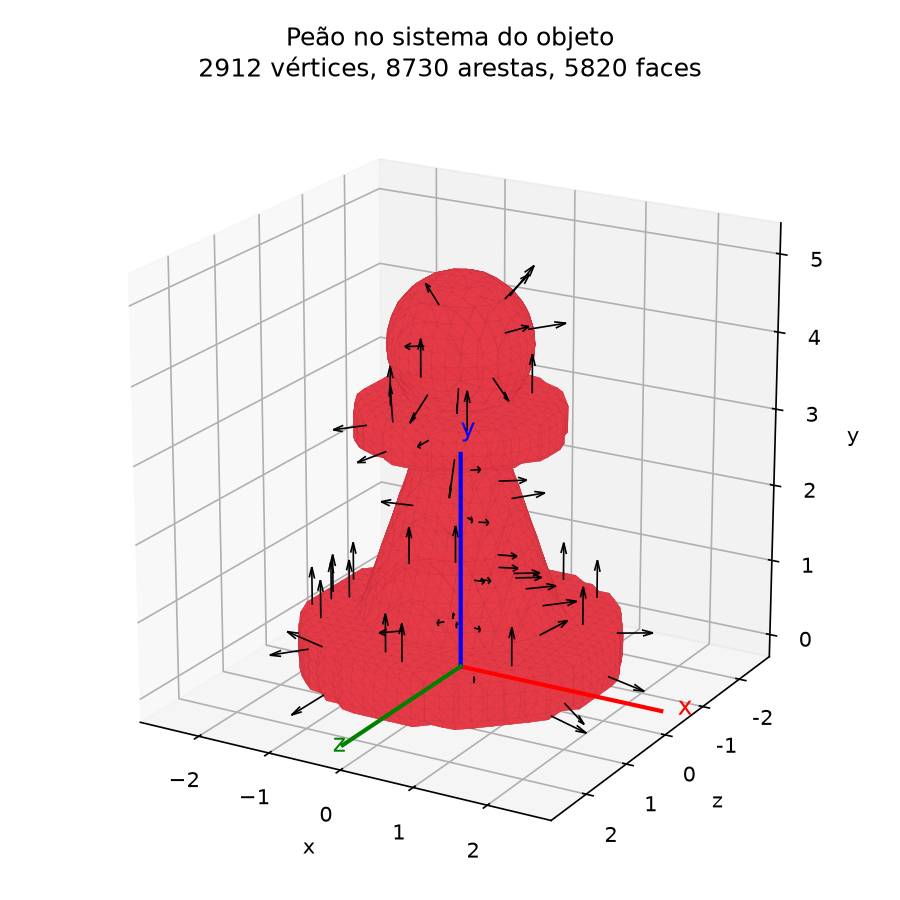
\includegraphics[width=\linewidth]{03-desenvolvimento/01-modelagem/peao.png}\caption{Peão}\end{subfigure}
\begin{subfigure}{0.32\linewidth}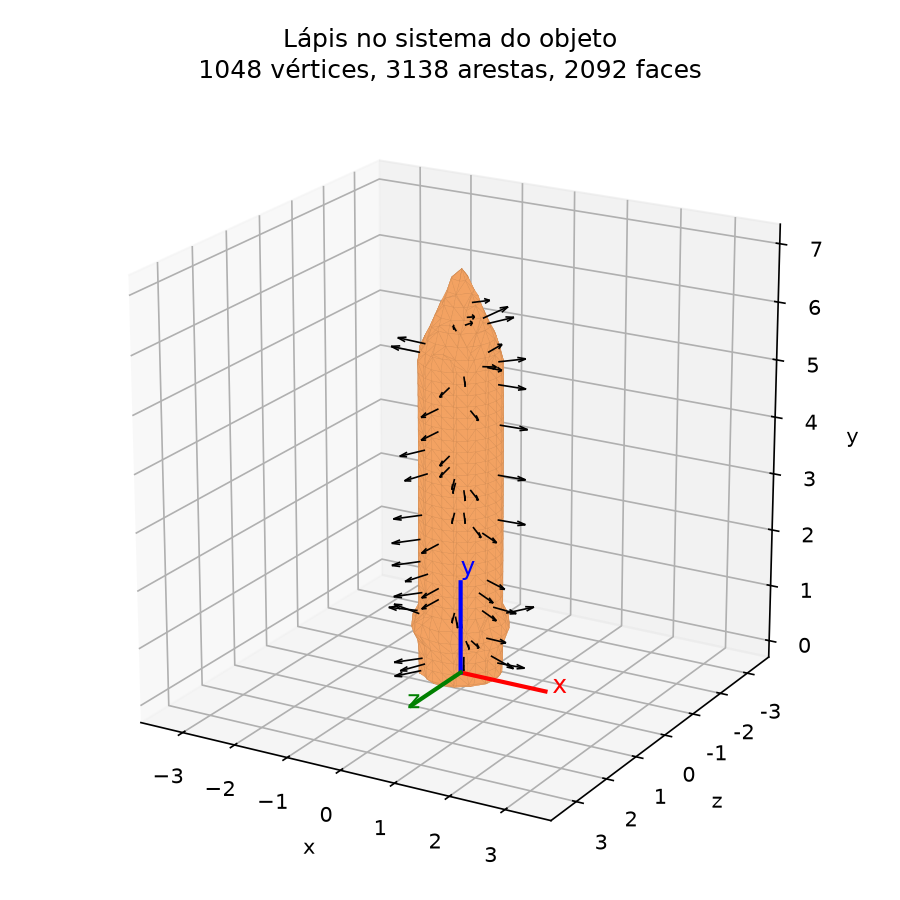
\includegraphics[width=\linewidth]{03-desenvolvimento/01-modelagem/lapis.png}\caption{Lápis}\end{subfigure}
\begin{subfigure}{0.32\linewidth}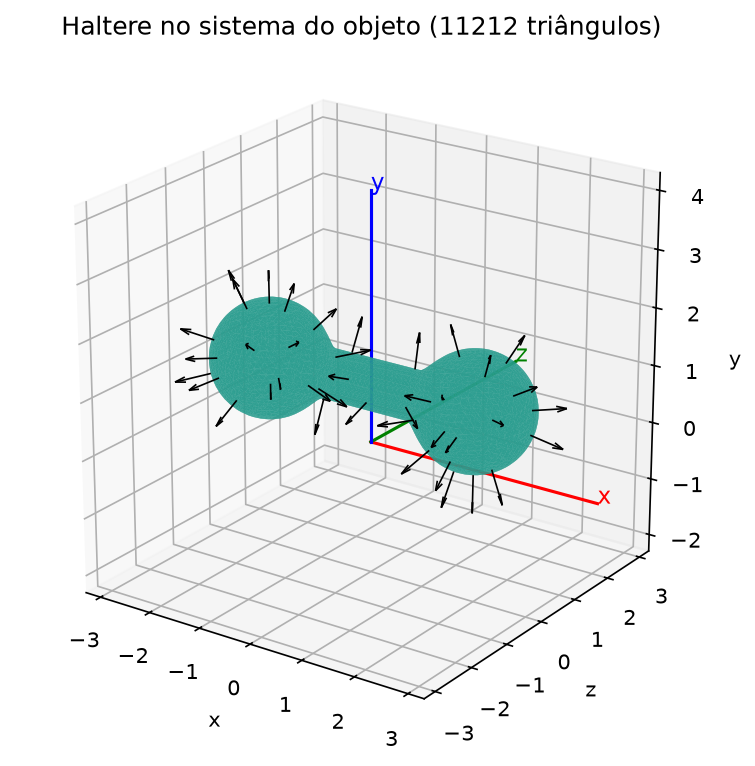
\includegraphics[width=\linewidth]{03-desenvolvimento/01-modelagem/haltere.png}\caption{Altere}\end{subfigure}\\[4pt]
\begin{subfigure}{0.32\linewidth}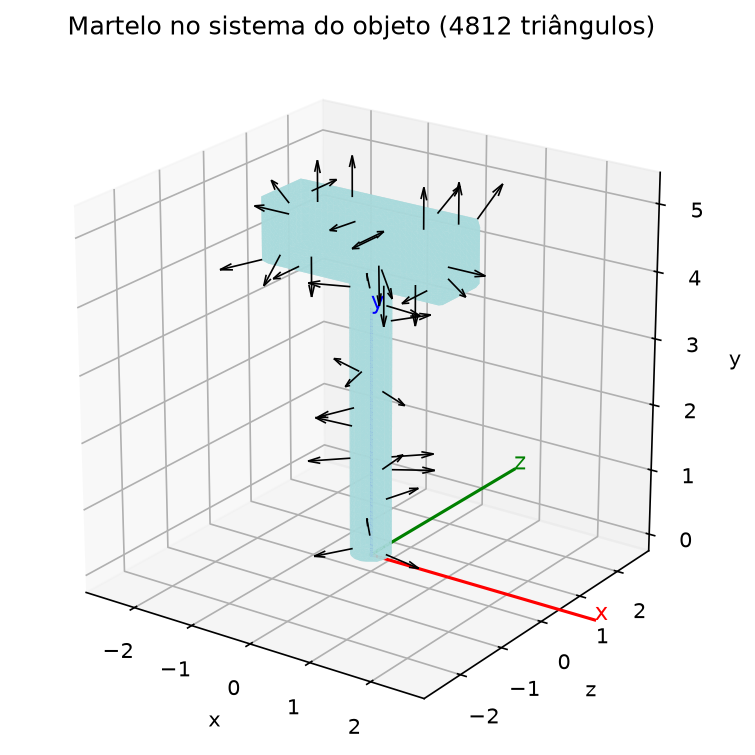
\includegraphics[width=\linewidth]{03-desenvolvimento/01-modelagem/martelo.png}\caption{Martelo}\end{subfigure}
\begin{subfigure}{0.32\linewidth}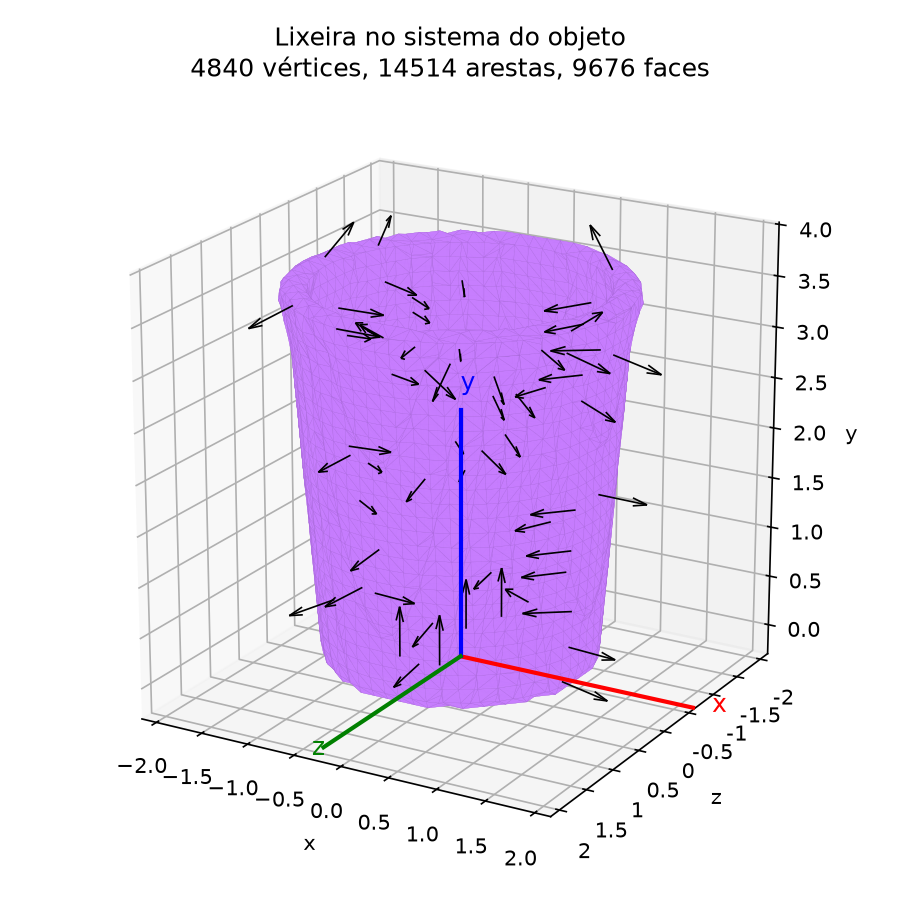
\includegraphics[width=\linewidth]{03-desenvolvimento/01-modelagem/lixeira.png}\caption{Lixeira}\end{subfigure}
\end{figure}

\subsection{Perguntas prováveis — Item 1}

\begin{pergunta}{Por que Marching Cubes e não um algoritmo próprio?}
O enunciado permite usar Marching Cubes por API. A vantagem é modelar cada objeto como uma função
implícita e combinar formas com CSG (união, interseção, subtração), o que é muito mais simples do que
montar triângulos à mão para formas como o toro da lixeira ou o altere.
\end{pergunta}

\begin{pergunta}{Como vocês garantem que a normal aponta para fora?}
A normal é $(B-A)\times(C-A)$; o sentido depende da ordem dos vértices. O Marching Cubes devolve os
triângulos numa ordem consistente que, com $F<0$ dentro, faz a normal apontar para fora. Conferimos
desenhando as normais como setas (\code{visualizar_objetos.py}) e, na prática, o back-face culling do
item 6 só funciona porque elas estão para fora: se estivessem invertidas, veríamos o interior dos objetos.
\end{pergunta}

\begin{pergunta}{Qual a diferença entre normal de face e normal de vértice?}
A de face é perpendicular ao triângulo e é usada no \textbf{back-face culling}. A de vértice é a soma
normalizada das normais das faces vizinhas e é usada na \textbf{iluminação}, para o sombreamento ficar
suave (Gouraud).
\end{pergunta}

\begin{pergunta}{O que acontece se aumentar a resolução do Marching Cubes?}
A grade fica mais fina, a malha ganha mais triângulos e a superfície fica mais fiel à função implícita
(menos facetada), mas o custo cresce com $\text{res}^3$ para avaliar $F$ e com o número de faces para
rasterizar. Usamos 80 no \code{main.py} e 50 nos gráficos de apoio.
\end{pergunta}

\begin{pergunta}{Como a lixeira fica oca?}
Subtração CSG: $\max(F_{\text{externo}}, -F_{\text{interno}})$. O cone interno começa um pouco acima
do fundo (sobra o fundo) e vai além do topo (abre a boca). A borda é um toro unido ao corpo.
\end{pergunta}

\begin{pergunta}{Como sabem que a malha não tem buracos?}
Pela característica de Euler: $V - A + F = 2$ nos 5 objetos, e $A = \frac32 F$ (cada aresta é
compartilhada por exatamente 2 triângulos).
\end{pergunta}

% =====================================================================
\novasecao
\section{Item 2 — Cena no sistema do mundo}
% =====================================================================

\begin{enunciado}
\textbf{Enunciado:} componha uma cena com os sólidos no sistema do mundo, sem sobreposição, usando
escala, rotação e translação; nenhuma componente de vértice pode passar de $|10|$; mostre em 3D.
\end{enunciado}

\subsection{Conceito: coordenadas homogêneas e transformações afins}

Escrevendo um ponto $(x,y,z)$ como $(x,y,z,1)$, \textbf{translação, rotação e escala viram
multiplicações por matrizes $4\times4$} e podem ser compostas numa só matriz (\arq{math_3d.py:4-57}):

\[
T = \begin{pmatrix} 1&0&0&t_x\\ 0&1&0&t_y\\ 0&0&1&t_z\\ 0&0&0&1 \end{pmatrix}
\qquad
S = \begin{pmatrix} s_x&0&0&0\\ 0&s_y&0&0\\ 0&0&s_z&0\\ 0&0&0&1 \end{pmatrix}
\]
\[
R_x(\theta) = \begin{pmatrix} 1&0&0&0\\ 0&\cos\theta&-\sin\theta&0\\ 0&\sin\theta&\cos\theta&0\\ 0&0&0&1 \end{pmatrix}
\quad
R_y(\theta) = \begin{pmatrix} \cos\theta&0&\sin\theta&0\\ 0&1&0&0\\ -\sin\theta&0&\cos\theta&0\\ 0&0&0&1 \end{pmatrix}
\]
\[
R_z(\theta) = \begin{pmatrix} \cos\theta&-\sin\theta&0&0\\ \sin\theta&\cos\theta&0&0\\ 0&0&1&0\\ 0&0&0&1 \end{pmatrix}
\]

Sem coordenadas homogêneas a translação seria uma soma ($\vetor p + \vetor t$) e não daria para
encadear tudo numa única matriz.

\subsection{A matriz do mundo}

\begin{conceito}{Matriz do mundo (\code{matriz_mundo}, \code{math_3d.py:60})}
\[
M = T \cdot R_z \cdot R_y \cdot R_x \cdot S,
\qquad \vetor p_{\text{mundo}} = M\,\vetor p_{\text{objeto}}
\]
Lida \textbf{da direita para a esquerda}: 1) escala, 2) rotação em $x$, $y$, $z$ (todas em torno da
origem do objeto), 3) translação até a posição na cena.
\end{conceito}

\textbf{A ordem importa} (o produto de matrizes não é comutativo): se transladássemos primeiro, a
rotação giraria o objeto em torno da origem \textbf{do mundo}, fazendo ele ``orbitar'' e sair do lugar.

\begin{figure}[H]\centering
\caption{Mesma rotação de $90^\circ$ e translação, em ordens diferentes}
\begin{tikzpicture}[scale=0.55]
  \begin{scope}
    \draw[->,gray] (-1,0)--(7,0) node[right]{$x$}; \draw[->,gray] (0,-1)--(0,6) node[above]{$y$};
    \fill[azulclaro!30,draw=azulclaro] (0,0) rectangle (2,1);
    \fill[peao!30,draw=peao] (4,1) rectangle (5,3);
    \draw[-{Stealth},thick] (2.2,0.5) to[bend left] node[above,font=\scriptsize]{$T\cdot R$} (3.9,2);
    \node[font=\footnotesize,align=center] at (3,-1.9) {$T\cdot R$: gira na origem\\ e depois translada \checkmark};
  \end{scope}
  \begin{scope}[xshift=15.5cm]
    \draw[->,gray] (-6,0)--(3,0) node[right]{$x$}; \draw[->,gray] (0,-1)--(0,6) node[above]{$y$};
    \fill[azulclaro!30,draw=azulclaro] (0,0) rectangle (2,1);
    \draw[dashed,azulclaro] (4,1) rectangle (6,2);
    \fill[peao!30,draw=peao] (-2,4) rectangle (-1,6);
    \draw[-{Stealth},thick,dashed] (5,2.1) to[bend right] node[pos=0.25,above right,font=\scriptsize]{gira em torno da origem} (-0.9,5);
    \node[font=\footnotesize,align=center] at (-1.5,-1.9) {$R\cdot T$: translada e depois gira\\ em torno da origem: ``orbita''};
  \end{scope}
\end{tikzpicture}
\end{figure}

Aplicação a todos os vértices de uma vez (\arq{math_3d.py:73}): \code{(homogeneos @ M.T)[:, :3]}, que
é o mesmo que $M\,\vetor p$ para cada ponto $\vetor p$.

\subsection{A cena montada}

\begin{table}[H]\centering\small
\caption{Configuração \code{CENA} (\code{cena.py:34}) e caixa resultante de cada objeto no mundo}
\begin{tabularx}{\linewidth}{@{}l c c c X@{}}
\toprule
\textbf{Objeto} & \textbf{Posição $(x,z)$} & \textbf{Rotação $(x,y,z)$} & \textbf{Escala} & \textbf{Caixa no mundo (mín .. máx)} \\
\midrule
Peão & $(-6{,}5;\ -4{,}5)$ & $(0, 0, 0)$ & 1,2 & $[-8{,}90;\ -2{,}00;\ -6{,}90]$ .. $[-4{,}10;\ 4{,}12;\ -2{,}10]$ \\
Lápis & $(-8{,}0;\ 0{,}5)$ & $(90^\circ, 45^\circ, 0)$ & 1,0 & $[-8{,}46;\ -2{,}00;\ 0{,}04]$ .. $[-3{,}00;\ -0{,}37;\ 5{,}50]$ \\
Altere & $(-1{,}5;\ -4{,}5)$ & $(0, 0, 90^\circ)$ & 0,9 & $[-3{,}30;\ -2{,}00;\ -5{,}40]$ .. $[-1{,}50;\ 3{,}40;\ -3{,}60]$ \\
Martelo & $(1{,}0;\ 3{,}2)$ & $(-90^\circ, -30^\circ, 0)$ & 1,0 & $[0{,}76;\ -2{,}00;\ -2{,}05]$ .. $[4{,}86;\ -1{,}00;\ 3{,}32]$ \\
Lixeira & $(3{,}5;\ -4{,}5)$ & $(0, 0, 0)$ & 1,1 & $[1{,}68;\ -2{,}00;\ -6{,}32]$ .. $[5{,}33;\ 2{,}11;\ -2{,}67]$ \\
\bottomrule
\end{tabularx}
\end{table}

Maior componente na cena: $\mathbf{8{,}90}$ (limite 10). As três transformações (escala, rotação e
translação) são de fato usadas, como o enunciado exige.

\textbf{Apoio no chão} — \code{montar_matriz} (\arq{cena.py:58}): primeiro aplica só $R\cdot S$,
descobre o $y$ mínimo do objeto já girado e escalado e escolhe
\[ t_y = Y_{\text{chão}} - y_{\min} = -2 - y_{\min}. \]
Assim todo objeto encosta exatamente em $y = -2$ (o $y$ mínimo de todas as caixas é $-2{,}00$).

\subsection{Validação automática}

\code{validar_cena} (\arq{cena.py:89}) confere a cena sozinha:
\begin{enumerate}
\item \textbf{Limite:} $\max_i |p_i| \le 10$ para toda componente de todo vértice.
\item \textbf{Sem sobreposição:} cada objeto é envolvido pela sua \textbf{AABB} (\emph{Axis-Aligned
  Bounding Box}, a menor caixa alinhada aos eixos que o contém). Duas caixas estão separadas se, em
  \textbf{pelo menos um eixo}, uma termina antes de a outra começar:
  \[ \exists\, k \in \{x,y,z\} : \quad \max_A[k] + \varepsilon < \min_B[k] \;\;\lor\;\; \max_B[k] + \varepsilon < \min_A[k], \qquad \varepsilon = 0{,}1. \]
  Se as caixas não se tocam, os objetos dentro delas também não.
\end{enumerate}
Se algo falhar, \code{imprimir_resumo} lança um erro: a cena nunca é renderizada inválida.

\subsection{Item 2b — mostrar em 3D}

\begin{figure}[H]\centering
\caption{Cena no sistema do mundo: origem (ponto preto), limite $|10|$ (tracejado), chão em $y=-2$ e a AABB de cada objeto (pontilhado)}
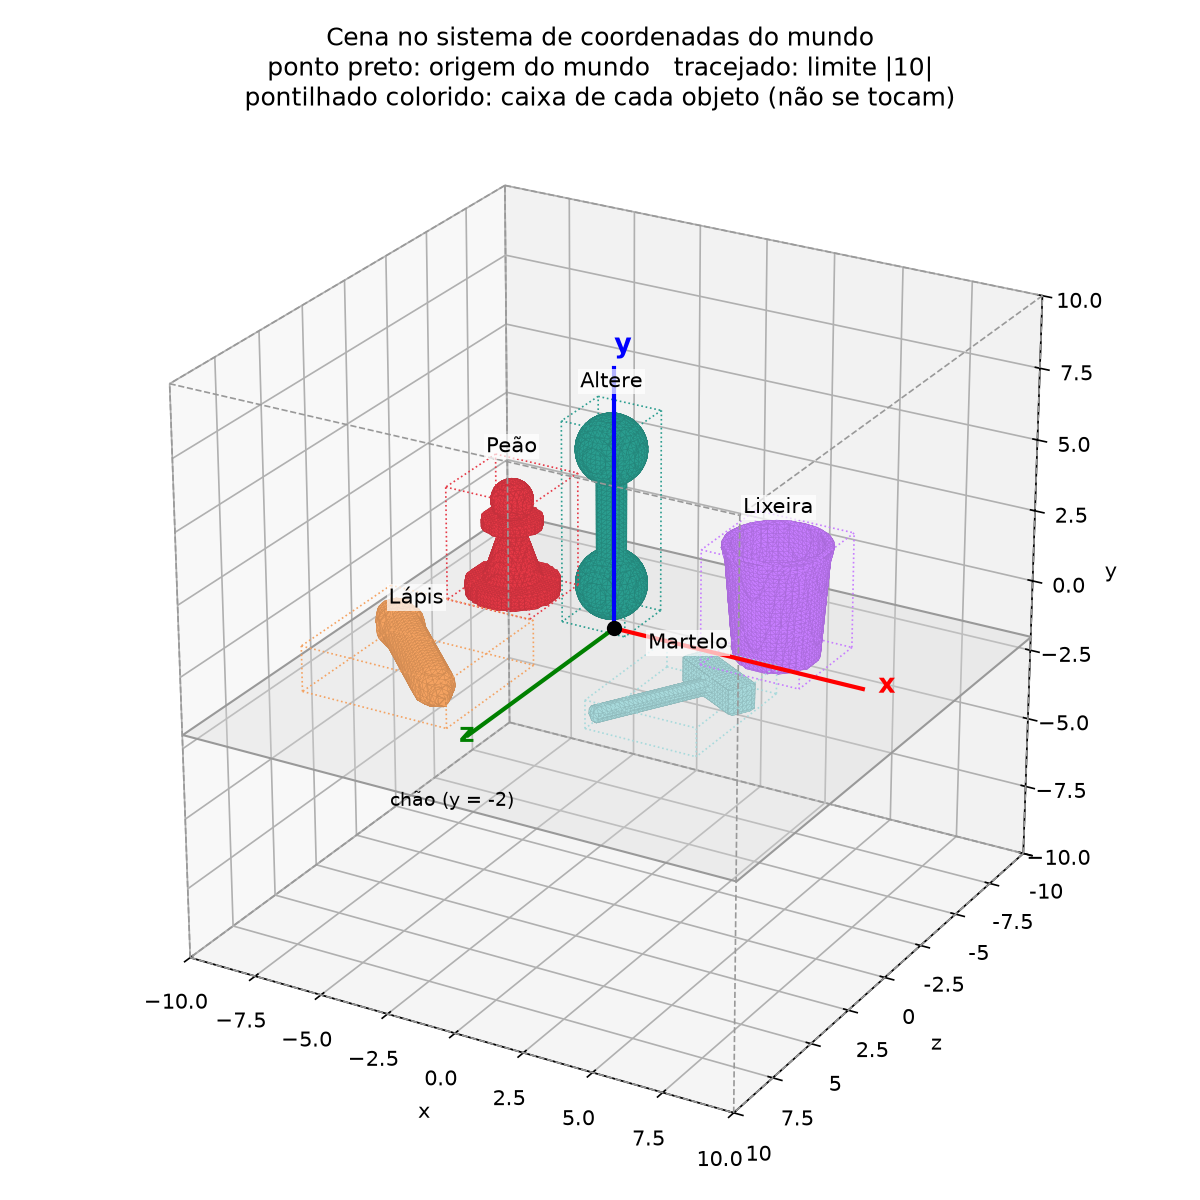
\includegraphics[width=0.5\linewidth]{03-desenvolvimento/02-cena/cena-mundo.png}
\end{figure}

\subsection{Perguntas prováveis — Item 2}

\begin{pergunta}{Por que usar matriz $4\times4$ e não $3\times3$?}
Porque a translação não é linear em 3D (é uma soma). Em coordenadas homogêneas ela vira
multiplicação, e assim escala, rotação e translação se combinam numa única matriz.
\end{pergunta}

\begin{pergunta}{Por que a ordem $T\cdot R\cdot S$? O que acontece se inverter?}
Escala e rotação precisam acontecer com o objeto na origem dele. Se transladar antes, a rotação seria
em torno da origem do mundo e o objeto mudaria de posição; a escala também multiplicaria a translação.
\end{pergunta}

\begin{pergunta}{Como garantem que não há interseção?}
Pelas AABBs: se as caixas envolventes não se cruzam, os objetos dentro delas também não. É um teste
conservador (pode recusar cenas que na verdade não se tocam), mas nunca aceita uma que se toca.
\end{pergunta}

\begin{pergunta}{Como uma rotação de $90^\circ$ em $z$ deixa o altere em pé?}
O altere foi modelado deitado ao longo de $x$. $R_z(90^\circ)$ leva o eixo $x$ para o eixo $y$, então a
barra fica vertical.
\end{pergunta}

\begin{pergunta}{Como as normais são transformadas para o mundo?}
Com a \textbf{inversa transposta} da parte $3\times3$ de $M$ (\code{matriz_normal}, \code{math_3d.py:83}):
$\vetor n' = (M_{3\times3}^{-1})^{T}\,\vetor n$. Com escala não uniforme, transformar a normal pela própria
$M$ a deixaria inclinada em relação à superfície; a inversa transposta preserva a perpendicularidade.
Na nossa cena as escalas são uniformes, mas o código já está correto para o caso geral.
\end{pergunta}

% =====================================================================
\novasecao
\section{Item 3 — Sistema de coordenadas da câmera}
% =====================================================================

\begin{enunciado}
\textbf{Enunciado:} escolha um eye; compute a base vetorial; transforme os objetos do mundo para a
câmera; mostre em 3D; marque a origem do mundo; o eye pode mudar e uma nova imagem deve ser gerada.
\end{enunciado}

\subsection{Conceito: base ortonormal da câmera}

\begin{conceito}{Base $(\vetor u, \vetor v, \vetor n)$ — \code{base_camera}, \code{math_3d.py:92}}
Dados \emph{eye} (observador), \emph{at} (ponto visado) e \emph{up} (``cima'' do mundo):
\[
\vetor n = \frac{eye - at}{\norm{eye - at}}, \qquad
\vetor u = \frac{up \times \vetor n}{\norm{up \times \vetor n}}, \qquad
\vetor v = \vetor n \times \vetor u.
\]
$\vetor n$ é o eixo $z$ da câmera e aponta \textbf{para trás} (do at para o eye); $\vetor u$ é o eixo $x$
(direita); $\vetor v$ é o eixo $y$ (cima). Os três são unitários e perpendiculares entre si, num sistema
de mão direita. A câmera \textbf{olha na direção $-z$}.
\end{conceito}

\begin{figure}[H]\centering
\caption{Base da câmera a partir de eye, at e up}
\begin{tikzpicture}[scale=1.1,>=Stealth]
  \coordinate (at) at (0,0);
  \coordinate (eye) at (4.2,1.6);
  \fill (at) circle (2pt) node[below left]{$at$};
  \fill[laranja] (eye) circle (2.5pt) node[left=3pt,text=black]{$eye$};
  \draw[dashed,gray] (at)--(eye) node[midway,above,sloped,font=\footnotesize]{direção de visada: $-\vetor n$};
  \draw[->,very thick,verde] (eye)--++(0.93*1.4,0.36*1.4) node[right]{$\vetor n$};
  \draw[->,very thick,peao] (eye)--++(0.36*1.2,-0.93*1.2) node[right]{$\vetor u$};
  \draw[->,very thick,azulclaro] (eye)--++(-0.15,1.4) node[above]{$\vetor v$};
  \draw[->,thick,gray] (-1.5,-0.3)--++(0,1.3) node[above,font=\footnotesize]{$up=(0,1,0)$};
\end{tikzpicture}
\end{figure}

Valores reais com a câmera principal ($eye = (9{,}75;\ 13;\ 6{,}5)$, $at = (0,0,0)$, $up = (0,1,0)$):
\[
\vetor u = (0{,}555;\ 0{,}000;\ -0{,}832) \qquad
\vetor v = (-0{,}618;\ 0{,}670;\ -0{,}412) \qquad
\vetor n = (0{,}557;\ 0{,}743;\ 0{,}371)
\]

O código trata os dois casos degenerados: $eye = at$ (sem direção de visada) e eye na mesma vertical do
at ($up \parallel \vetor n$, produto vetorial nulo); nos dois lança um erro explicativo.

\subsection{Matriz de visualização (look-at)}

\begin{conceito}{Matriz de visualização — \code{look_at}, \code{math_3d.py:119}}
\[
V = R \cdot T(-eye) =
\begin{pmatrix}
u_x & u_y & u_z & -\vetor u\cdot eye\\
v_x & v_y & v_z & -\vetor v\cdot eye\\
n_x & n_y & n_z & -\vetor n\cdot eye\\
0&0&0&1
\end{pmatrix}
\]
Primeiro translada o eye para a origem; depois roda o mundo para os eixos da câmera coincidirem com
$x$, $y$, $z$ (as linhas da rotação são $\vetor u$, $\vetor v$, $\vetor n$).
\end{conceito}

Para a câmera principal:
\[
V = \begin{pmatrix}
0{,}555 & 0 & -0{,}832 & 0\\
-0{,}618 & 0{,}670 & -0{,}412 & 0\\
0{,}557 & 0{,}743 & 0{,}371 & -17{,}502\\
0&0&0&1
\end{pmatrix},
\qquad 17{,}502 = \norm{eye - at}.
\]
As duas primeiras translações dão 0 porque o at é a origem: o eye está exatamente sobre o eixo $\vetor n$.

\subsection{Itens 3a--3e na prática}

\begin{itemize}
\item \textbf{3a} — \code{main.py} e \code{visualizar_camera.py} imprimem $\vetor u, \vetor v, \vetor n$ no terminal.
\item \textbf{3b} — \code{aplicar_transformacao(view, vertices_mundo)} leva todos os vértices para a câmera.
\item \textbf{3c} — \code{visualizar_camera.py} desenha os sólidos nesse sistema, com os eixos
  $\vetor u, \vetor v, \vetor n$ saindo da origem (que é o eye) e o volume de visão (pirâmide tracejada).
\item \textbf{3d} — origem do mundo: ponto preto em $V\,(0,0,0,1)^T$ no \code{visualizar_camera.py}; na imagem
  rasterizada, uma \textbf{cruz laranja} (\code{desenhar_origem_mundo}, \arq{main.py:87}).
\item \textbf{3e} — o eye muda pela linha de comando: \texttt{-{}-eye X Y Z} em \code{main.py},
  \code{visualizar_camera.py} e \code{visualizar_projecao.py}. O \code{main.py} também gera sempre uma
  \textbf{Tela 2} com um segundo eye $(26, 18, 28)$.
\end{itemize}

\begin{figure}[H]\centering
\caption{A cena no sistema da câmera com dois eyes diferentes (item 3e)}
\begin{subfigure}{0.48\linewidth}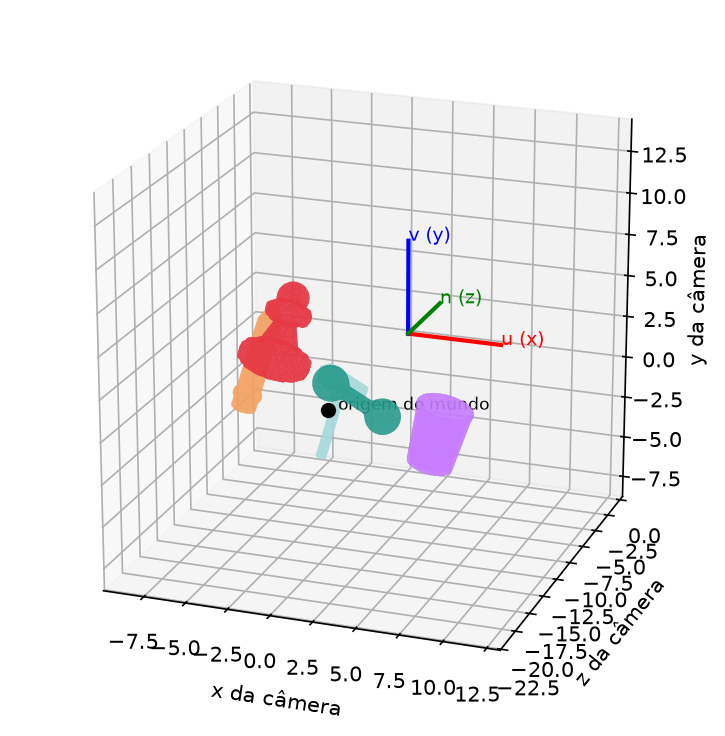
\includegraphics[width=\linewidth]{03-desenvolvimento/03-camera/eye1.png}\caption{$eye = (9{,}75;\ 13;\ 6{,}5)$}\end{subfigure}\hfill
\begin{subfigure}{0.48\linewidth}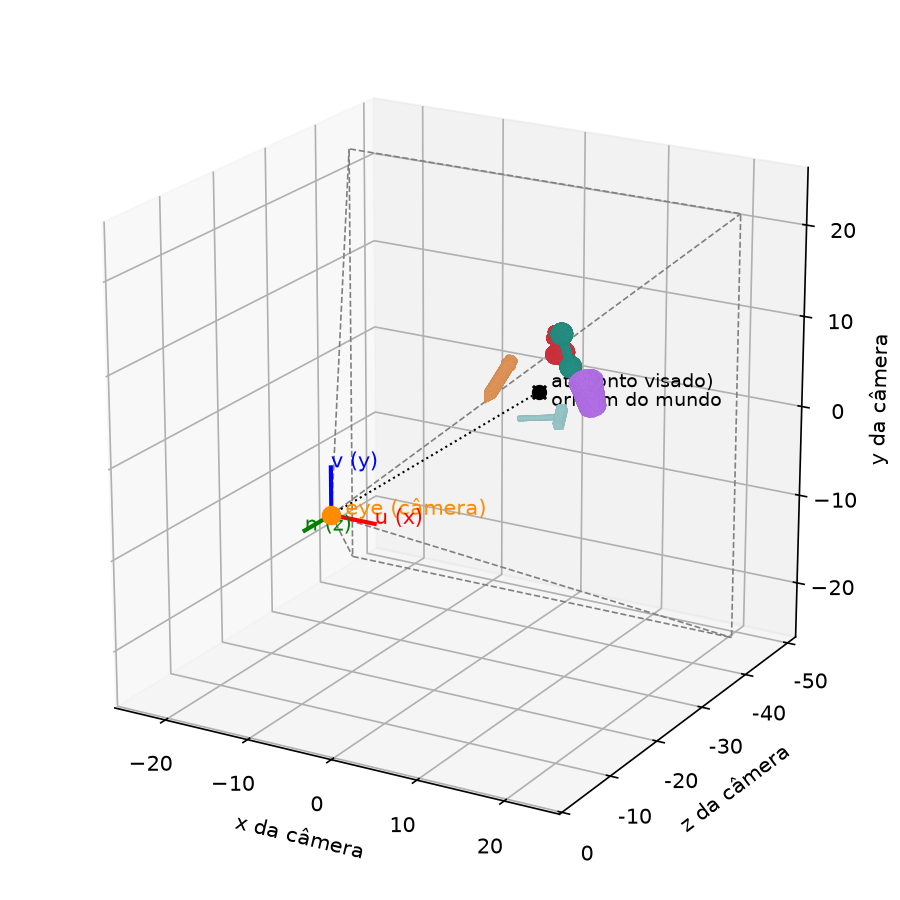
\includegraphics[width=\linewidth]{03-desenvolvimento/03-camera/eye2.png}\caption{$eye = (26;\ 18;\ 28)$}\end{subfigure}
\end{figure}

\subsection{Perguntas prováveis — Item 3}

\begin{pergunta}{Por que $\vetor n$ aponta do at para o eye, e não o contrário?}
Convenção de sistema de mão direita (OpenGL): com $\vetor u$ para a direita e $\vetor v$ para cima, o
$z$ positivo sai da tela em direção ao observador; logo a câmera olha para $-z$.
\end{pergunta}

\begin{pergunta}{Por que precisa do vetor up?}
Só eye e at definem a direção de visada, mas a câmera ainda poderia girar em torno dela. O up fixa
essa rotação: $\vetor u = up\times\vetor n$ fica horizontal e $\vetor v$ fica o mais próximo possível do
``cima'' do mundo.
\end{pergunta}

\begin{pergunta}{Por que $\vetor v = \vetor n\times\vetor u$ não precisa ser normalizado?}
Porque $\vetor n$ e $\vetor u$ já são unitários e perpendiculares:
$\norm{\vetor n\times\vetor u} = \norm{\vetor n}\,\norm{\vetor u}\,\sin 90^\circ = 1$.
\end{pergunta}

\begin{pergunta}{O que acontece se o eye estiver exatamente acima do at?}
O up fica paralelo a $\vetor n$, o produto vetorial dá zero e a base não existe. O código detecta e
lança erro (seria preciso escolher outro up).
\end{pergunta}

\begin{pergunta}{Qual a relação entre a matriz $V$ e a base?}
As linhas da parte $3\times3$ são $\vetor u$, $\vetor v$ e $\vetor n$; a última coluna é
$-(\vetor u\cdot eye,\ \vetor v\cdot eye,\ \vetor n\cdot eye)$, a translação do eye para a origem já
escrita na nova base. Como é rotação + translação, ela preserva distâncias e ângulos (transformação rígida).
\end{pergunta}

\begin{pergunta}{Como a imagem muda com outro eye?}
Só a matriz $V$ muda; a cena no mundo é a mesma. Por isso basta recalcular $\vetor u, \vetor v, \vetor n$
e reprojetar.
\end{pergunta}

% =====================================================================
\novasecao
\section{Item 4 — Projeção em perspectiva e volume de visão}
% =====================================================================

\begin{enunciado}
\textbf{Enunciado:} projeção perspectiva dos sólidos no volume de visão, polígono a polígono, na
janela de projeção; polígonos não visíveis não vão para o plano; arestas e faces de um sólido com a
mesma cor, sólidos diferentes com cores diferentes; apresentar em 2D na janela (com o 3D junto).
\end{enunciado}

\subsection{Conceito: projeção perspectiva}

Por \textbf{semelhança de triângulos}, um ponto $(x,y,z)$ da câmera projeta numa janela a distância $d$ em
\[ x' = \frac{d\,x}{-z}, \qquad y' = \frac{d\,y}{-z}. \]
Objetos mais distantes ($|z|$ maior) ficam menores: é isso que dá a sensação de profundidade.

\begin{figure}[H]\centering
\caption{Semelhança de triângulos na projeção perspectiva (vista lateral, plano $yz$)}
\begin{tikzpicture}[scale=1.0,>=Stealth]
  \draw[->,gray] (0.5,0)--(-8,0) node[left]{$-z$};
  \draw[->,gray] (0,-0.5)--(0,3.2) node[above]{$y$};
  \fill[laranja] (0,0) circle (2.5pt) node[below right,text=black]{eye};
  \draw[very thick,azulclaro] (-3,-0.3)--(-3,2.6) node[above,font=\footnotesize]{janela};
  \fill[peao] (-7,2.4) circle (2.5pt) node[above,text=black]{$(y,\ z)$};
  \draw[dashed] (0,0)--(-7,2.4);
  \fill[azulclaro] (-3,1.0286) circle (2.2pt) node[left,text=black,font=\footnotesize]{$y'$};
  \draw[dotted] (-7,0)--(-7,2.4);
  \draw[<->] (0,-0.9)--(-3,-0.9) node[midway,below,font=\footnotesize]{$d$};
  \draw[<->] (0,-1.6)--(-7,-1.6) node[midway,below,font=\footnotesize]{$-z$};
  \node[font=\small] at (-5.2,-2.6) {$\dfrac{y'}{d} = \dfrac{y}{-z} \;\Rightarrow\; y' = \dfrac{d\,y}{-z}$};
\end{tikzpicture}
\end{figure}

\subsection{A matriz de projeção}

\begin{conceito}{Matriz de projeção perspectiva — \code{projecao_perspectiva}, \code{math_3d.py:137}}
\[
P = \begin{pmatrix}
\dfrac{f}{\text{aspecto}} & 0 & 0 & 0\\[6pt]
0 & f & 0 & 0\\[4pt]
0 & 0 & \dfrac{far+near}{near-far} & \dfrac{2\,far\,near}{near-far}\\[8pt]
0 & 0 & -1 & 0
\end{pmatrix},
\qquad f = \cot\!\left(\frac{fov}{2}\right).
\]
\end{conceito}

Com $fov = 58^\circ$, aspecto 1, near $=0{,}1$ e far $=100$:
\[
P = \begin{pmatrix}
1{,}804 & 0 & 0 & 0\\
0 & 1{,}804 & 0 & 0\\
0 & 0 & -1{,}002 & -0{,}2\\
0 & 0 & -1 & 0
\end{pmatrix}
\]

\begin{itemize}
\item $f = \cot(29^\circ) \approx 1{,}804$ é o $d$ da aula, para uma janela de altura 2 (de $-1$ a $1$).
\item A última linha faz $\mathbf{w = -z}$. A \textbf{divisão perspectiva} (\code{divisao_perspectiva},
  \arq{math_3d.py:157}) divide $x, y, z$ por $w$:
  \[ x_{\text{NDC}} = \frac{x_{\text{clip}}}{w} = \frac{f\,x}{-z}, \]
  exatamente o $x' = d\,x/(-z)$ da aula.
\item A 3ª linha mapeia a profundidade: $z = -near \mapsto z_{\text{NDC}} = -1$ e
  $z = -far \mapsto z_{\text{NDC}} = +1$. Esse $z_{\text{NDC}}$ é o que vai para o Z-buffer.
\end{itemize}

O resultado são as \textbf{NDC} (\emph{Normalized Device Coordinates}), em $[-1,1]^3$. Depois,
\code{ndc_para_pixel} (\arq{main.py:27}) leva para a tela:
\[
x_{\text{pixel}} = \frac{x_{\text{NDC}} + 1}{2}\cdot\text{res},
\qquad
y_{\text{pixel}} = \frac{1 - y_{\text{NDC}}}{2}\cdot\text{res}
\quad\text{(inverte $y$: na imagem a linha 0 fica em cima).}
\]

\subsection{Volume de visão e recorte}

O \textbf{volume de visão} (\emph{frustum}) é a pirâmide truncada entre os planos near e far, limitada
pelo fov. Em \textbf{coordenadas de recorte} (antes de dividir por $w$), um ponto está dentro quando
\[ -w \le x \le w, \qquad -w \le y \le w, \qquad -w \le z \le w; \]
cada desigualdade é um dos 6 planos.

\begin{figure}[H]\centering
\caption{Volume de visão (frustum) entre os planos near e far}
\begin{tikzpicture}[scale=0.9,>=Stealth]
  \coordinate (E) at (0,0);
  \coordinate (n1) at (1.5,0.75); \coordinate (n2) at (1.5,-0.75);
  \coordinate (f1) at (7,3.5); \coordinate (f2) at (7,-3.5);
  \fill[azulclaro!10] (n1)--(f1)--(f2)--(n2)--cycle;
  \draw[gray,dashed] (E)--(n1) (E)--(n2);
  \draw[thick,azulclaro] (n1)--(f1) (n2)--(f2);
  \draw[very thick,verde] (n1)--(n2) node[below,font=\footnotesize]{near};
  \draw[very thick,peao] (f1)--(f2) node[below,font=\footnotesize]{far};
  \fill[laranja] (E) circle (2.5pt) node[left,text=black]{eye};
  \draw[->] (E)--(8,0) node[right]{$-z$};
  \draw (0.8,0) arc (0:26.57:0.8); \node[font=\scriptsize] at (1.15,0.25) {$\frac{fov}{2}$};
  \fill[peao] (4,1) circle (2pt); \node[font=\footnotesize,right] at (4,1) {dentro: desenha};
  \fill[gray] (3.6,3.3) circle (2pt); \node[font=\footnotesize,left] at (3.6,3.3) {fora (todos os vértices): descarta};
  \fill[gray] (-0.8,1.2) circle (2pt); \node[font=\footnotesize,left] at (-0.8,1.2) {atrás do near: descarta};
\end{tikzpicture}
\end{figure}

\code{face_no_volume_de_visao} (\arq{math_3d.py:164}) descarta o \textbf{triângulo inteiro} quando:
\begin{enumerate}
\item \textbf{algum vértice está atrás do near} ($z < -w$): depois da divisão por $w$, ele ``passaria
  para o outro lado'' da câmera e deformaria o triângulo;
\item \textbf{os 3 vértices estão fora do mesmo plano} (esquerda, direita, baixo, cima ou far). Se
  estivessem fora de planos diferentes, o triângulo ainda poderia cruzar a tela, então é mantido.
\end{enumerate}
Faces parcialmente fora que sobrevivem são cortadas na rasterização, que só pinta pixels dentro da tela.

\subsection{Polígonos não visíveis e cores}

Antes de projetar, cada face passa por dois filtros: \textbf{recorte} (acima) e \textbf{back-face
culling} (Seção~\ref{sec:culling}). O \code{main.py} mostra no título de cada imagem quantas faces
foram desenhadas, quantas caíram fora do volume e quantas estavam de costas.

Cada sólido tem uma cor única. Faces e arestas usam \textbf{a mesma cor do sólido}: as arestas são
desenhadas com a equação da reta na cor iluminada dos próprios vértices (\code{desenhar_aresta}, \arq{main.py:65}).

\subsection{Item 4a — 3D e 2D juntos}

\code{visualizar_projecao.py} mostra dois painéis:
\begin{itemize}
\item \textbf{3D:} os sólidos em coordenadas de câmera, a \textbf{janela de projeção} (quadrado tracejado
  no plano $z = -d$) e, sobre ela, os triângulos visíveis já projetados. Uma reta pontilhada liga o eye ao
  centro de cada sólido e cruza a janela exatamente no ponto projetado.
\item \textbf{2D:} a mesma janela vista de frente.
\end{itemize}
Como o matplotlib não tem Z-buffer, só nesse gráfico de apoio os triângulos são ordenados do mais
distante para o mais próximo (\textbf{algoritmo do pintor}).

\subsection{Perguntas prováveis — Item 4}

\begin{pergunta}{Por que precisa da coordenada $w$ e da divisão perspectiva?}
A projeção perspectiva divide por $z$, e divisão não é uma operação linear: não cabe numa matriz. O
truque é a matriz copiar $-z$ para $w$; a divisão por $w$ acontece depois, separadamente.
\end{pergunta}

\begin{pergunta}{O que são NDC?}
Coordenadas normalizadas em $[-1,1]$ nos três eixos, independentes da resolução. O mesmo NDC vira 200,
400 ou 800 pixels só mudando o \code{res} em \code{ndc_para_pixel}.
\end{pergunta}

\begin{pergunta}{Qual a diferença entre o recorte e o back-face culling?}
O recorte tira o que está \textbf{fora do campo de visão} (atrás do near, além do far ou fora das
laterais). O culling tira o que está \textbf{dentro} do campo de visão mas \textbf{de costas} para a câmera.
\end{pergunta}

\begin{pergunta}{Por que o recorte é feito antes da divisão por $w$?}
Porque um vértice atrás da câmera tem $w$ negativo; dividir por $w$ inverteria o sinal de $x$ e $y$ e
ele apareceria espelhado na tela. Em coordenadas de recorte o teste é só comparar com $\pm w$.
\end{pergunta}

\begin{pergunta}{Vocês recortam o triângulo (Sutherland--Hodgman)?}
Não: o triângulo é aceito ou descartado inteiro. O que passa do limite da tela é cortado na
rasterização (só pixels dentro da imagem são pintados). Na nossa cena, com todos os objetos à frente da
câmera, isso não causa perda visível.
\end{pergunta}

\begin{pergunta}{Para que servem o near e o far?}
Limitam a profundidade do volume de visão e definem o mapeamento de $z$ para $[-1,1]$. O near não pode
ser 0, porque a divisão por $z$ explodiria.
\end{pergunta}

% =====================================================================
\novasecao
\section{Item 5 — Iluminação de Phong}
% =====================================================================

\begin{enunciado}
\textbf{Enunciado:} aplique iluminação aos vértices dos polígonos visíveis, calculando as componentes
ambiente, difusa e especular para obter o RGB dos vértices/pixels.
\end{enunciado}

\subsection{Conceito}

\begin{conceito}{Modelo de reflexão de Phong (1975)}
\[
I \;=\; \underbrace{k_a\, I_l\, O}_{\text{ambiente}}
\;+\; \underbrace{k_d\, I_l\, O\, \max(\vetor N\cdot\vetor L,\ 0)}_{\text{difusa (Lambert)}}
\;+\; \underbrace{k_s\, I_l\, \max(\vetor R\cdot\vetor V,\ 0)^{\alpha}}_{\text{especular}},
\qquad
\vetor R = 2(\vetor N\cdot\vetor L)\,\vetor N - \vetor L
\]
$O$ é a cor do objeto e $I_l$ a cor da luz. Todos os vetores são unitários.
\end{conceito}

\begin{figure}[H]\centering
\caption{Vetores do modelo de Phong num ponto da superfície}
\begin{tikzpicture}[scale=1.3,>=Stealth]
  \fill[gray!15] (-3,-0.4) rectangle (3,0); \draw[thick] (-3,0)--(3,0);
  \coordinate (P) at (0,0);
  \coordinate (N) at (0,2.2); \coordinate (L) at (-1.6,1.6); \coordinate (R) at (1.6,1.6); \coordinate (V) at (2.2,0.9);
  \draw[->,very thick,azul] (P)--(0,2.2) node[above]{$\vetor N$};
  \draw[->,very thick,laranja] (P)--(-1.6,1.6) node[left=6pt]{$\vetor L$ (até a luz)};
  \draw[->,very thick,peao] (P)--(1.6,1.6) node[above right]{$\vetor R$ (reflexão)};
  \draw[->,very thick,verde] (P)--(2.2,0.9) node[right]{$\vetor V$ (até o eye)};
  \pic[draw,angle radius=0.9cm,"$\theta$",angle eccentricity=1.3,font=\footnotesize] {angle=N--P--L};
  \pic[draw,angle radius=1.4cm,"$\phi$",angle eccentricity=1.2,font=\footnotesize] {angle=V--P--R};
  \fill (P) circle (1.5pt);
  \fill[laranja] (-1.95,1.95) circle (3pt) node[above,font=\footnotesize]{luz};
\end{tikzpicture}
\end{figure}

\begin{itemize}
\item \textbf{Ambiente:} luz indireta, constante; evita que o lado sem luz fique preto.
\item \textbf{Difusa (Lei do cosseno de Lambert):} proporcional a $\cos\theta = \vetor N\cdot\vetor L$.
  Não depende do observador.
\item \textbf{Especular:} o brilho. É forte quando o observador está perto da direção de reflexão
  ($\cos\phi = \vetor R\cdot\vetor V$ perto de 1). O expoente $\alpha$ controla o tamanho da mancha.
\end{itemize}

\subsection{Implementação}

\code{calcular_iluminacao_phong} (\arq{illumination.py:11}):

\begin{table}[H]\centering\small
\begin{tabular}{@{}l l@{}}
\toprule
\textbf{Parâmetro} & \textbf{Valor} \\
\midrule
$k_a,\ k_d,\ k_s$ & $0{,}5;\ 0{,}8;\ 0{,}4$ \\
Expoente de brilho $\alpha$ & 32 \\
Cor da luz $I_l$ & branca $(1,1,1)$ \\
Posição da luz & $(5, 20, 15)$ — \code{POSICAO_LUZ}, \code{cena.py:26} \\
Observador & o eye da câmera atual \\
\bottomrule
\end{tabular}
\end{table}

\begin{itemize}
\item Ambiente e difusa são multiplicadas pela cor do objeto; \textbf{a especular não}, então o brilho
  sai branco (como num objeto de plástico).
\item Se $\vetor N\cdot\vetor L \le 0$ (luz atrás da superfície), difusa e especular são zero.
\item O resultado é limitado a $[0, 1]$ com \code{np.clip}.
\item O cálculo é feito \textbf{no sistema do mundo}, com as normais transformadas pela inversa
  transposta (\code{normais_mundo}, \arq{main.py:145}).
\end{itemize}

\textbf{Só nos vértices visíveis, e uma vez só} (\arq{main.py:184-195}): Phong roda \textbf{depois} do
recorte e do culling, só para vértices de faces visíveis, como o enunciado pede. Um vértice é
compartilhado por cerca de 6 triângulos, então a cor fica guardada num dicionário \code{cores} e é
calculada uma única vez. Calcular a cor nos vértices e interpolar dentro do triângulo é o
\textbf{sombreamento de Gouraud}.

\subsection{Perguntas prováveis — Item 5}

\begin{pergunta}{Qual a diferença entre o modelo de Phong e o sombreamento de Phong?}
O \textbf{modelo} de Phong é a equação de iluminação (ambiente + difusa + especular). O
\textbf{sombreamento} de Phong interpola as \emph{normais} e aplica o modelo em cada pixel. Nós usamos o
modelo de Phong com \textbf{sombreamento de Gouraud}: aplicamos a equação nos vértices e interpolamos
as \emph{cores} com a baricêntrica.
\end{pergunta}

\begin{pergunta}{Por que a difusa não depende do observador?}
Uma superfície difusa (lambertiana) espalha a luz igualmente em todas as direções, então parece igual
de qualquer ângulo. Só depende de quanta luz chega, que é proporcional a $\cos\theta = \vetor N\cdot\vetor L$.
\end{pergunta}

\begin{pergunta}{O que o expoente 32 faz?}
Controla o quão concentrado é o brilho. $\cos^{32}\phi$ cai muito rápido longe de $\vetor R$, gerando
uma mancha pequena e nítida; com expoente 2 a mancha seria grande e espalhada.
\end{pergunta}

\begin{pergunta}{Como se calcula $\vetor R$?}
Decompondo $\vetor L$ na parte paralela à normal, $(\vetor N\cdot\vetor L)\vetor N$, e espelhando a parte
perpendicular: $\vetor R = 2(\vetor N\cdot\vetor L)\vetor N - \vetor L$.
\end{pergunta}

\begin{pergunta}{Por que normalizar os vetores?}
Porque o produto escalar só é igual ao cosseno do ângulo quando os vetores são unitários:
$\vetor a\cdot\vetor b = \norm{\vetor a}\norm{\vetor b}\cos\theta$.
\end{pergunta}

\begin{pergunta}{Por que a especular aparece branca?}
Ela multiplica só a cor da luz (branca), não a do objeto: imita materiais como plástico, em que o
reflexo especular tem a cor da fonte de luz.
\end{pergunta}

% =====================================================================
\novasecao
\section{Item 6 — Rasterização}
% =====================================================================

\begin{enunciado}
\textbf{Enunciado:} rasterize em pelo menos 3 resoluções; antes, elimine polígonos ocultos usando a
normal e o eixo $z$ da câmera; depois, calcule a cor dos pixels por interpolação baricêntrica; use a
rasterização de retas (livro, subseção 5.2.1) e de polígonos (par-ímpar com scan-line).
\end{enunciado}

\subsection{Três resoluções}

\code{RESOLUCOES_TELA = [200, 400, 800]} (\arq{main.py:17}). A Tela 1 do \code{main.py} mostra as
três lado a lado; com \texttt{-{}-salvar} gera os PNGs no relatório. Como tudo até as NDC é igual, só a
conversão para pixel muda, e dá para comparar o efeito do \textbf{aliasing} (serrilhado) na resolução baixa.

\begin{figure}[H]\centering
\caption{Imagem final rasterizada em três resoluções (câmera principal)}
\begin{subfigure}{0.32\linewidth}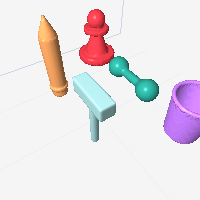
\includegraphics[width=\linewidth]{04-simulacoes/eye1-200.png}\caption{$200\times200$}\end{subfigure}
\begin{subfigure}{0.32\linewidth}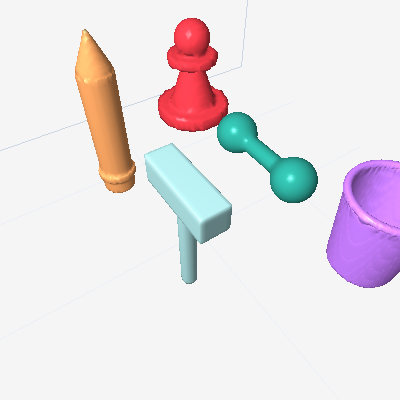
\includegraphics[width=\linewidth]{04-simulacoes/eye1-400.png}\caption{$400\times400$}\end{subfigure}
\begin{subfigure}{0.32\linewidth}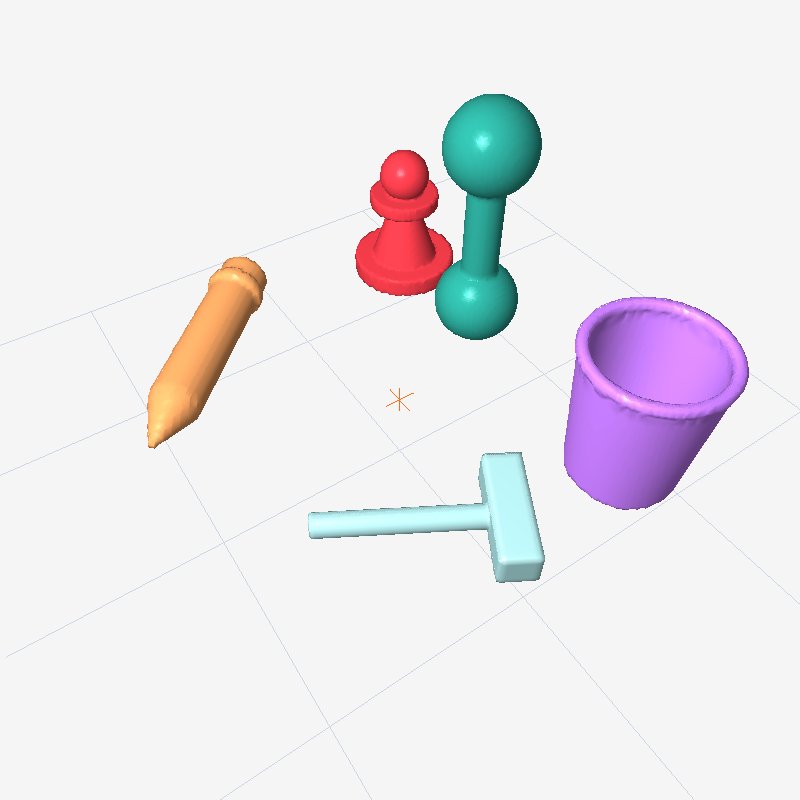
\includegraphics[width=\linewidth]{04-simulacoes/eye1-800.png}\caption{$800\times800$}\end{subfigure}
\end{figure}

\subsection{Back-face culling}\label{sec:culling}

\begin{conceito}{Teste de face visível — \code{face_voltada_para_camera}, \code{math_3d.py:198}}
\[
\text{desenha a face} \iff \vetor n\cdot\vetor v < 0,
\qquad \vetor v = \text{vértice} - eye = \text{vértice}\ \ (\text{na câmera o eye é a origem})
\]
$\vetor n$ é a normal da face \textbf{no sistema da câmera}: objeto $\to$ mundo pela inversa transposta,
mundo $\to$ câmera pela parte $3\times3$ de $V$ (\arq{main.py:149-150}).
\end{conceito}

\begin{figure}[H]\centering
\caption{Faces de frente ($\vetor n\cdot\vetor v<0$) e de costas ($\vetor n\cdot\vetor v\ge0$) num objeto}
\begin{tikzpicture}[scale=1.1,>=Stealth]
  \fill[laranja] (-4,0) circle (3pt) node[below,text=black]{eye};
  \draw[thick,fill=lixeira!15] (0,0) circle (1.3);
  \foreach \a in {135,180,225}{
    \draw[->,thick,verde] (\a:1.3)--(\a:2.1);
  }
  \foreach \a in {0,45,315}{
    \draw[->,thick,peao] (\a:1.3)--(\a:2.1);
  }
  \draw[->,dashed,gray] (-4,0)--(158:1.3) node[midway,above,font=\footnotesize]{$\vetor v$};
  \node[verde,font=\footnotesize,align=center] at (-1.9,1.9) {de frente\\ $\vetor n\cdot\vetor v<0$};
  \node[peao,font=\footnotesize,align=center] at (2.6,1.5) {de costas\\ $\vetor n\cdot\vetor v\ge0$\\ (descartada)};
\end{tikzpicture}
\end{figure}

\textbf{Por que não testar só o sinal de $n_z$ (o eixo $z$ da câmera)?} Em projeção
\textbf{perspectiva} a direção de visada muda de face para face; só no centro da imagem ela coincide com
o eixo $z$. Testar apenas $n_z$ descartaria, perto das bordas, faces quase de lado que ainda são
visíveis. O teste $\vetor n\cdot\vetor v$ é o geral e, no centro da imagem
($\vetor v \approx (0, 0, -1)$), se reduz a $n_z > 0$: a condição do enunciado com o eixo $z$ da câmera.

Em objetos fechados, o culling elimina cerca de metade das faces, uma economia grande antes da etapa
cara (rasterizar pixel a pixel).

\subsection{Rasterização de retas — equação da reta}

\code{rasterizar_reta} (\arq{rasterizer.py:14}) é o algoritmo dado em aula. Calcula $m = dy/dx$ e
$b = y_1 - m\,x_1$ e anda de 1 em 1 no eixo que mais varia:

\begin{lstlisting}
dx, dy = x2 - x1, y2 - y1
if abs(dx) > abs(dy):                  # mais deitada: anda em x
    m = dy / dx;  b = y1 - m * x1
    for x in range(x1, x2 + passo, passo):
        produz_fragmento(x, m * x + b)
else:                                  # mais em pé: anda em y
    for y in range(y1, y2 + passo, passo):
        produz_fragmento((y - b) / m, y)   # vertical (dx = 0) fica separada
\end{lstlisting}

\code{produz_fragmento} (\arq{rasterizer.py:5}) pega a \textbf{parte inteira} de $x$ e de $y$: o pixel
é o que contém o ponto, com centro em $(\lfloor x\rfloor + 0{,}5,\ \lfloor y\rfloor + 0{,}5)$.

\begin{figure}[H]\centering
\caption{Equação da reta de $(0,0)$ a $(5,2)$: cada pixel é a parte inteira de $y = 0{,}4\,x$}
\begin{tikzpicture}[scale=0.8]
  \draw[gray!40] (0,0) grid (6,3);
  \foreach \x/\y in {0/0,1/0,2/0,3/1,4/1,5/2}{
    \fill[azulclaro!60] (\x,\y) rectangle ++(1,1);
  }
  \draw[very thick,peao] (0.5,0.5)--(5.5,2.5);
  \node[font=\footnotesize,right] at (6.3,1.5) {$m = \dfrac{dy}{dx} = \dfrac{2}{5}$};
\end{tikzpicture}
\end{figure}

Além do quadro, o código converte os extremos para inteiros (o laço sempre termina), usa passo $-1$
quando a reta vai para a esquerda ou para baixo, trata a reta vertical ($dx = 0$, $m$ infinito) à parte e
devolve os pontos na ordem de $p_1$ para $p_2$. É usado nas \textbf{arestas de cada face}
(\code{desenhar_aresta}, \arq{main.py:65}), na cor iluminada dos vértices, interpolando cor e $z$ ao
longo da reta (isso também \textbf{fecha frestas} que o scan-line pode deixar nas bordas), e na
\textbf{grade do chão} e na \textbf{cruz da origem} (\code{desenhar_reta_3d_no_zbuffer}, \arq{main.py:40}).

\subsection{Rasterização de polígonos — scan-line par-ímpar}

\code{scan_line_par_impar} (\arq{rasterizer.py:72}):
\begin{enumerate}
\item Acha $y_{\min}$ e $y_{\max}$ do polígono (limitados à tela).
\item Para cada linha horizontal $y$ (\emph{scan line}), calcula a interseção com cada aresta:
  \[ x = x_1 + (y - y_1)\,\frac{x_2 - x_1}{y_2 - y_1}. \]
\item A condição $y_1 \le y < y_2$ (intervalo semiaberto) evita contar duas vezes um vértice
  compartilhado e ignora arestas horizontais.
\item Ordena as interseções e \textbf{pinta entre os pares} (1ª--2ª, 3ª--4ª, \ldots): regra
  \textbf{par-ímpar}.
\item \code{ceil} no início e \code{floor} no fim do intervalo: só entram pixels cujo centro está dentro.
\end{enumerate}

\begin{figure}[H]\centering
\caption{Scan-line par-ímpar: entre a 1ª e a 2ª interseção está dentro}
\begin{tikzpicture}[scale=0.8]
  \fill[lapis!20,draw=lapis!80!black,thick] (0,0)--(7,1)--(5,4.5)--(3,2.2)--(1,4)--cycle;
  \draw[azul,thick] (-0.8,3)--(8,3) node[right,font=\footnotesize]{scan line $y$};
  \foreach \x/\l in {0.778/1,2.111/2,3.696/3,5.857/4}{
    \fill[peao] (\x,3) circle (2.5pt) node[above,font=\scriptsize,text=black]{\l};
  }
  \draw[line width=3pt,verde,opacity=0.6] (0.778,3)--(2.111,3);
  \draw[line width=3pt,verde,opacity=0.6] (3.696,3)--(5.857,3);
  \node[font=\footnotesize,align=left] at (10.3,1.2) {\textcolor{verde}{pinta}: 1--2 e 3--4\\ não pinta: 2--3 (fora)};
\end{tikzpicture}
\end{figure}

\subsection{Interpolação baricêntrica}

\begin{conceito}{Coordenadas baricêntricas — \code{coordenadas_baricentricas}, \code{rasterizer.py:53}}
Para um pixel $P$ no triângulo $ABC$:
\[
\alpha = \frac{\text{área}(P,B,C)}{\text{área}(A,B,C)}, \qquad
\beta = \frac{\text{área}(A,P,C)}{\text{área}(A,B,C)}, \qquad
\gamma = 1 - \alpha - \beta,
\]
\[
\text{área}(A,B,C) = \tfrac12\,\big|\,x_A(y_B - y_C) + x_B(y_C - y_A) + x_C(y_A - y_B)\,\big|.
\]
$P = \alpha A + \beta B + \gamma C$, com $\alpha+\beta+\gamma = 1$; $P$ está dentro se $\alpha,\beta,\gamma \ge 0$.
\end{conceito}

\begin{figure}[H]\centering
\caption{Cada peso é a área do subtriângulo oposto ao vértice, dividida pela área total}
\begin{tikzpicture}[scale=1.2]
  \coordinate (A) at (0,0); \coordinate (B) at (5,0.3); \coordinate (C) at (2,3.4); \coordinate (P) at (2.3,1.2);
  \fill[peao!30] (P)--(B)--(C)--cycle;
  \fill[verde!30] (A)--(P)--(C)--cycle;
  \fill[azulclaro!30] (A)--(B)--(P)--cycle;
  \draw[thick] (A)--(B)--(C)--cycle;
  \draw (P)--(A) (P)--(B) (P)--(C);
  \fill (P) circle (2pt) node[above right,font=\footnotesize]{$P$};
  \node[below left] at (A) {$A$}; \node[below right] at (B) {$B$}; \node[above] at (C) {$C$};
  \node[font=\footnotesize] at (3.15,1.6) {$\alpha$};
  \node[font=\footnotesize] at (1.45,1.5) {$\beta$};
  \node[font=\footnotesize] at (2.45,0.5) {$\gamma$};
\end{tikzpicture}
\end{figure}

Com elas o \code{main.py} interpola (\arq{main.py:206-218}):
\[
\text{cor}_P = \alpha\,\text{cor}_A + \beta\,\text{cor}_B + \gamma\,\text{cor}_C \quad\text{(Gouraud)},
\qquad
z_P = \alpha\,z_A + \beta\,z_B + \gamma\,z_C \quad\text{(para o Z-buffer)}.
\]

\subsection{Z-buffer (extra, além do pedido)}

Matriz $\text{res}\times\text{res}$ iniciada com $+\infty$ (\arq{main.py:128}). Para cada pixel:
\[
\text{se } z_P < \text{zbuffer}[y, x]:\qquad \text{zbuffer}[y,x] \leftarrow z_P,\quad \text{imagem}[y,x] \leftarrow \text{cor}_P.
\]
Resolve a visibilidade \textbf{entre objetos} e \textbf{dentro de objetos côncavos} (por exemplo o
interior da lixeira), o que o culling sozinho não resolve. \code{Z_BIAS = 0.005} dá uma folga nas
retas da grade e da origem para evitar \emph{z-fighting}.

\subsection{Elementos extras na imagem}
\begin{itemize}
\item \textbf{Grade do chão} em $y = -2$, de $-10$ a $10$, a cada 5 unidades (\arq{main.py:97}).
\item \textbf{Cruz laranja na origem do mundo} (item 3d) (\arq{main.py:87}).
\item \textbf{Título} com a contagem: total de faces, desenhadas, fora do volume e de costas.
\end{itemize}

\subsection{Perguntas prováveis — Item 6}

\begin{pergunta}{Por que andar em $x$ quando $|dx| > |dy|$ e em $y$ no caso contrário?}
Para não deixar buracos. Andando sempre em $x$, uma reta em pé ($m > 1$) subiria mais de um pixel em
$y$ a cada passo e ficaria pontilhada. Andando no eixo que mais varia, cada passo muda no máximo 1 pixel
no outro eixo.
\end{pergunta}

\begin{pergunta}{E a reta vertical?}
Nela $dx = 0$ e $m$ é infinito, então $x = (y - b)/m$ não pode ser calculado. O código trata à parte:
$x$ fica fixo e $y$ anda de 1 em 1.
\end{pergunta}

\begin{pergunta}{Qual a diferença para o Bresenham?}
A equação da reta calcula $m\,x + b$ em ponto flutuante a cada passo e trunca o resultado. O Bresenham
(aprimoramento) decide o próximo pixel só com soma e subtração de inteiros e uma variável de erro, e
escolhe o pixel mais perto da reta (arredonda). De $(0,0)$ a $(5,2)$, ele daria $(2,1)$ e $(4,2)$ onde a
equação da reta dá $(2,0)$ e $(4,1)$.
\end{pergunta}

\begin{pergunta}{Explique a regra par-ímpar.}
Traçando uma linha horizontal pelo polígono, ela entra e sai alternadamente. Ordenando as interseções,
os trechos entre a 1ª e a 2ª, a 3ª e a 4ª etc. estão dentro.
\end{pergunta}

\begin{pergunta}{Por que o intervalo semiaberto $y_1 \le y < y_2$?}
Num vértice onde duas arestas se encontram, a scan line tocaria as duas e contaria a interseção duas
vezes, quebrando a paridade. O intervalo semiaberto conta cada vértice uma vez só e descarta arestas
horizontais ($y_1 = y_2$), que causariam divisão por zero.
\end{pergunta}

\begin{pergunta}{O que são coordenadas baricêntricas?}
Os pesos $(\alpha,\beta,\gamma)$ que escrevem $P$ como combinação dos vértices, $P = \alpha A + \beta B +
\gamma C$, com soma 1. Cada peso é a razão entre a área do subtriângulo oposto ao vértice e a área
total: quanto mais perto de $A$, maior $\alpha$.
\end{pergunta}

\begin{pergunta}{Por que fazer culling se já tem Z-buffer?}
Desempenho: o culling descarta cerca de metade das faces com um único produto escalar, antes da etapa
cara (Phong + rasterização por pixel). O Z-buffer resolve o resto: objetos na frente de outros e
partes côncavas de um mesmo objeto.
\end{pergunta}

\begin{pergunta}{O culling basta para remover superfícies ocultas?}
Só para um objeto \textbf{convexo} sozinho. Na lixeira (côncava) ou quando um objeto está na frente de
outro, faces de frente também podem estar escondidas; por isso o Z-buffer.
\end{pergunta}

\begin{pergunta}{Qual o efeito da resolução?}
Em $200\times200$ cada pixel cobre uma área maior da cena: as bordas ficam serrilhadas (aliasing) e
triângulos pequenos podem sumir. Em $800\times800$ a imagem fica mais fiel, mas o custo cresce com o
número de pixels (16 vezes mais que em $200\times200$).
\end{pergunta}

\begin{pergunta}{Por que desenhar as arestas por cima das faces?}
O enunciado pede arestas da mesma cor do sólido, e o scan-line com \code{ceil}/\code{floor} pode deixar
frestas de um pixel entre triângulos vizinhos; a aresta fecha essas frestas.
\end{pergunta}

\begin{pergunta}{Por que o renderizador demora?}
É Python puro, pixel a pixel, por fidelidade didática aos algoritmos da aula. Uma implementação real
vetorizaria com NumPy ou usaria a GPU.
\end{pergunta}

% =====================================================================
\novasecao
\section{Como executar}
% =====================================================================

\begin{lstlisting}[language=bash]
python3 -m venv .venv
source .venv/bin/activate
pip install -r requirements.txt

python3 visualizar_objetos.py                  # item 1e: cada sólido no seu sistema
python3 visualizar_cena.py                     # item 2b: cena no mundo
python3 cena.py                                # item 2:  imprime as caixas e valida
python3 visualizar_camera.py                   # item 3:  cena no sistema da câmera
python3 visualizar_camera.py --eye 26 18 28    # item 3e: outro eye
python3 visualizar_projecao.py                 # item 4a: 3D + janela de projeção
python3 main.py                                # itens 4, 5, 6: imagem final (alguns minutos)
python3 main.py --eye 26 18 28                 # item 3e na imagem final
python3 main.py --salvar eye1                  # salva eye1-200/400/800.png no relatório
\end{lstlisting}

\textbf{Roteiro sugerido para a apresentação:} seguir a ordem acima, que mostra a evolução objeto
$\to$ mundo $\to$ câmera $\to$ projeção $\to$ imagem final, na mesma ordem dos itens do enunciado. Para o
item 3e, rodar \code{visualizar_camera.py} com dois eyes (é rápido) em vez do \code{main.py}.

% =====================================================================
\section{Limitações conhecidas (e como responder sobre elas)}
% =====================================================================

\begin{table}[H]\centering\small
\begin{tabularx}{\linewidth}{@{}>{\raggedright\arraybackslash}p{4.6cm} X@{}}
\toprule
\textbf{Limitação} & \textbf{Resposta} \\
\midrule
Recorte descarta o triângulo inteiro, sem Sutherland--Hodgman & Os objetos ficam todos à frente da câmera; triângulos parcialmente fora das laterais são cortados pelo limite da tela na rasterização. Recortar polígonos seria a evolução natural. \\
Interpolação de cor no espaço da tela (não corrigida por perspectiva) & Gouraud clássico. Em triângulos pequenos (malha fina do Marching Cubes) a diferença é imperceptível. Já a profundidade $z_{\text{NDC}}$ é afim no espaço da tela, então a interpolação dela está correta. \\
Teste de sobreposição por AABB & É conservador: pode recusar uma cena que não se toca, mas nunca aceita uma que se toca. \\
Malha depende do Marching Cubes por API & Permitido explicitamente pelo item 1b. \\
Renderização lenta & Python puro por pixel, para seguir os algoritmos da aula literalmente. \\
Z-buffer não foi pedido & É um extra; o culling pedido está implementado e é aplicado antes. \\
\bottomrule
\end{tabularx}
\end{table}

% =====================================================================
\novasecao
\section{Banco de perguntas rápidas}
% =====================================================================

{\small
\begin{longtable}{@{}>{\raggedright\arraybackslash}p{5.3cm} >{\raggedright\arraybackslash}p{6.6cm} l@{}}
\toprule
\textbf{Pergunta} & \textbf{Resposta curta} & \textbf{Onde} \\
\midrule
\endhead
Quais os sistemas de coordenadas? & objeto $\to$ mundo $\to$ câmera $\to$ recorte $\to$ NDC $\to$ tela & Seção 1 \\
O que retorna a função do sólido? & dicionário com vértices, arestas, faces, normais de face e de vértice, cor & \code{modeling.py:29} \\
Como combinar formas implícitas? & união $=\min$, interseção $=\max$, subtração $=\max(A,-B)$ & \code{primitives.py:20} \\
Normal de um triângulo? & $(B-A)\times(C-A)$ normalizado & \code{modeling.py:50} \\
Como transformar normais? & inversa transposta da parte $3\times3$ & \code{math_3d.py:83} \\
Ordem da matriz do mundo? & $T\,R_z\,R_y\,R_x\,S$ (escala, rotação, translação) & \code{math_3d.py:60} \\
Como checar $|10|$? & $\max|\text{vértices}| \le 10$ & \code{cena.py:101} \\
Como checar sobreposição? & AABBs separadas em algum eixo & \code{cena.py:106} \\
Base da câmera? & $\vetor n = \frac{eye-at}{\|\cdot\|}$, $\vetor u = \frac{up\times\vetor n}{\|\cdot\|}$, $\vetor v = \vetor n\times\vetor u$ & \code{math_3d.py:92} \\
Para onde a câmera olha? & $-z$ & \code{math_3d.py:152} \\
O que faz $w = -z$? & permite a divisão perspectiva $x' = d\,x/(-z)$ & \code{math_3d.py:153} \\
Teste do volume de visão? & $-w \le x, y, z \le w$ & \code{math_3d.py:164} \\
Teste de culling? & $\vetor n\cdot\vetor v < 0$ na câmera & \code{math_3d.py:198} \\
Componentes de Phong? & $k_a O$, $\ k_d O (\vetor N\cdot\vetor L)$, $\ k_s (\vetor R\cdot\vetor V)^{32}$ & \code{illumination.py:11} \\
Fórmula de $\vetor R$? & $2(\vetor N\cdot\vetor L)\vetor N - \vetor L$ & \code{illumination.py:38} \\
Gouraud ou Phong shading? & Gouraud (cor nos vértices, interpolada) & \code{main.py:184} \\
Algoritmo de reta? & equação da reta, anda no eixo que mais varia & \code{rasterizer.py:14} \\
Algoritmo de polígono? & scan-line par-ímpar & \code{rasterizer.py:72} \\
Baricêntrica? & razão de áreas, $\alpha+\beta+\gamma = 1$ & \code{rasterizer.py:53} \\
Resoluções? & 200, 400, 800 & \code{main.py:17} \\
NDC $\to$ pixel? & $x = \frac{x+1}{2}\text{res}$, $\ y = \frac{1-y}{2}\text{res}$ & \code{main.py:27} \\
Visibilidade entre objetos? & Z-buffer (menor $z$ vence) & \code{main.py:213} \\
Como provar que a malha é fechada? & $V - A + F = 2$ e $A = \frac32 F$ & Seção 2.6 \\
\bottomrule
\end{longtable}
}

% =====================================================================
\section{Glossário}
% =====================================================================

\begin{description}[style=nextline,leftmargin=0.6cm,font=\bfseries\color{azul}]
\item[AABB] Caixa envolvente alinhada aos eixos.
\item[Back-face culling] Descarte de faces voltadas para longe do observador.
\item[CSG] Modelagem por combinação booleana de sólidos (união, interseção, subtração).
\item[Coordenadas homogêneas] $(x, y, z, w)$; permitem translação e perspectiva como matrizes.
\item[Coordenadas de recorte] Resultado de $P\,V\,M\,\vetor p$, antes da divisão por $w$.
\item[Divisão perspectiva] Dividir $x, y, z$ por $w$; leva das coordenadas de recorte para as NDC.
\item[Frustum / volume de visão] Pirâmide truncada entre near e far que a câmera enxerga.
\item[Gouraud] Iluminação calculada nos vértices e interpolada nos pixels.
\item[Marching Cubes] Algoritmo que extrai uma malha de triângulos de um campo escalar.
\item[NDC] Coordenadas normalizadas do dispositivo, em $[-1,1]^3$.
\item[Par-ímpar] Regra de preenchimento: dentro se cruzar a borda um número ímpar de vezes.
\item[Superfície implícita] Superfície definida por $F(x,y,z) = 0$.
\item[Z-buffer] Matriz com a profundidade do que já foi pintado em cada pixel.
\item[Z-fighting] Cintilação quando duas superfícies têm profundidades quase iguais.
\end{description}

\end{document}
